\documentclass[10pt]{article}
\usepackage[margin=0.90in]{geometry}
\linespread{1.02}
\usepackage[T1]{fontenc}
\usepackage{lmodern}
\usepackage{microtype}
\usepackage{amsmath,amssymb,amsthm}
\usepackage{booktabs,longtable,graphicx,multirow}
\usepackage{xcolor}
\usepackage{enumitem}
\usepackage[authoryear,round]{natbib}
\usepackage[colorlinks=true,linkcolor=blue!55!black,citecolor=blue!55!black,urlcolor=blue!55!black]{hyperref}
\urlstyle{same}

\newtheorem{proposition}{Proposition}
\newtheorem{theorem}{Theorem}
\newtheorem{corollary}{Corollary}
\newtheorem{definition}{Definition}

\raggedbottom
\setlength{\textfloatsep}{12pt plus 3pt minus 2pt}
\setlength{\floatsep}{9pt plus 2pt minus 2pt}
\renewcommand{\topfraction}{.92}
\renewcommand{\floatpagefraction}{.80}
\renewcommand{\textfraction}{.07}

% AUTO-GENERATED BY exp/v2/verify_all_numbers.py — DO NOT HAND-EDIT NUMBERS!

\newcommand{\MirageSGRatioD}{3.89\times}
\newcommand{\MirageSGUnpD}{2.464}
\newcommand{\MirageSGSameD}{0.633}
\newcommand{\MirageSGConfoundD}{74.3\%}
\newcommand{\MirageSGRatioSNR}{3.48\times}
\newcommand{\MirageSGUnpSNR}{5.33}
\newcommand{\MirageSGSameSNR}{1.53}
\newcommand{\MirageSGConfoundSNR}{71.3\%}
\newcommand{\OrthResCos}{0.150}
\newcommand{\OrthRtrCos}{0.238}
\newcommand{\GPQATokCut}{47.6\%}
\newcommand{\SGTokCut}{21.0\%}
\newcommand{\LegacyFourteenErr}{27/64 (42.2\%)}
\newcommand{\LegacyEightErr}{32/136 (23.5\%)}
\newcommand{\MirageGPQARatioD}{3.67\times}
\newcommand{\MirageGPQAUnpD}{2.141}
\newcommand{\MirageGPQASameD}{0.584}
\newcommand{\MirageGPQARatioSNR}{4.40\times}
\newcommand{\MirageGPQAUnpSNR}{5.82}
\newcommand{\MirageGPQASameSNR}{1.32}

\newcommand{\TableGatePhase}{%
\begin{table}[tbp]
\centering\small
\caption{Retention--Drift Phase Transition across gate sizes $n_g$ and $z$-score thresholds $z_{\min}$ (10,000 simulated 4-generation chains per cell, $A=2$ attempts/gen, paired flip rate $p_{\mathrm{flip}}=0.15$ calibrated to Qwen3-14B). Unthresholded $n_g=40$ gates yield 27.0\% false 4-generation survival and a $+9.57$\,pp Goodhart gap even for slightly harmful editors; strict gates ($z_{\min}\ge 1.65$) eliminate drift but require $n_g\ge 256$ for competent editors to retain edits reliably.}
\label{tab:gate-phase}
\footnotesize\setlength{\tabcolsep}{4.5pt}
\begin{tabular}{@{}lrrrrrrr@{}}
\toprule
Editor Regime & $n_g$ & $z_{\min}$ & $\mathrm{SE}_g$ (\%) & $P(\text{surv}_4)$ (\%) & False Ret. (\%) & $\mathbb{E}[\Delta_{\mathrm{true}}]$ (pp) & Goodhart Gap (pp) \\
\midrule
Weak/Null ($\mu=-0.4$\,pp) & 40 & 0.00 & 6.12 & 27.00 & 60.5 & $-0.50$ & $+9.57$ \\
 & 40 & 1.00 & 6.12 & 0.45 & 55.6 & $-0.05$ & $+3.41$ \\
 & 40 & 1.65 & 6.12 & 0.02 & 54.7 & $-0.01$ & $+1.18$ \\
 & 40 & 2.00 & 6.12 & 0.00 & 53.6 & $-0.00$ & $+0.61$ \\
 & 120 & 0.00 & 3.54 & 24.37 & 56.5 & $-0.29$ & $+5.27$ \\
 & 120 & 1.00 & 3.54 & 0.45 & 48.4 & $+0.01$ & $+1.88$ \\
 & 120 & 1.65 & 3.54 & 0.01 & 44.6 & $+0.02$ & $+0.66$ \\
 & 120 & 2.00 & 3.54 & 0.00 & 43.7 & $+0.01$ & $+0.35$ \\
 & 256 & 0.00 & 2.42 & 21.93 & 52.5 & $-0.10$ & $+3.38$ \\
 & 256 & 1.00 & 2.42 & 0.47 & 41.0 & $+0.07$ & $+1.23$ \\
 & 256 & 1.65 & 2.42 & 0.01 & 35.0 & $+0.04$ & $+0.45$ \\
 & 256 & 2.00 & 2.42 & 0.00 & 32.8 & $+0.02$ & $+0.25$ \\
\midrule
Competent ($\mu=+1.5$\,pp) & 40 & 0.00 & 6.12 & 47.35 & 18.8 & $+5.47$ & $+9.57$ \\
 & 40 & 1.00 & 6.12 & 3.17 & 12.4 & $+1.97$ & $+5.13$ \\
 & 40 & 1.65 & 6.12 & 0.10 & 8.3 & $+0.72$ & $+2.20$ \\
 & 40 & 2.00 & 6.12 & 0.02 & 6.1 & $+0.38$ & $+1.26$ \\
 & 120 & 0.00 & 3.54 & 56.58 & 14.8 & $+6.67$ & $+4.78$ \\
 & 120 & 1.00 & 3.54 & 8.28 & 7.5 & $+3.31$ & $+3.38$ \\
 & 120 & 1.65 & 3.54 & 0.68 & 3.7 & $+1.53$ & $+1.75$ \\
 & 120 & 2.00 & 3.54 & 0.13 & 2.6 & $+0.94$ & $+1.16$ \\
 & 256 & 0.00 & 2.42 & 62.62 & 12.0 & $+7.49$ & $+2.71$ \\
 & 256 & 1.00 & 2.42 & 15.88 & 4.9 & $+4.70$ & $+2.33$ \\
 & 256 & 1.65 & 2.42 & 3.00 & 1.8 & $+2.68$ & $+1.48$ \\
 & 256 & 2.00 & 2.42 & 0.89 & 1.2 & $+1.89$ & $+1.10$ \\
\bottomrule
\end{tabular}
\end{table}%
}

\newcommand{\TableExpBMain}{%
\begin{table}[tbp]
\centering\small
\caption{Experiment~B: Training-free weight editing on held-out SuperGPQA-Hard (Qwen3.5-35B-A3B, Brief-CoT, cap 768, $n=128\times 2=256$ paired evaluations per arm; base accuracy 18.75\%, base $\mathrm{acc}|\mathrm{fin}=45.7\%$, mean 631.6 tokens). Every single weight and steering edit (9/9) produces $\Delta_{\mathrm{comp}}>0$ alongside $\Delta_{\mathrm{reas}}<0$.}
\label{tab:expb-main}
\footnotesize\setlength{\tabcolsep}{3.0pt}
\resizebox{\linewidth}{!}{%
\begin{tabular}{@{}lrrrrrrr@{}}
\toprule
Intervention Arm & Acc (\%) & $\Delta$ [95\% CI] (pp) & $p$ & $\Delta_{\mathrm{comp}}$ & $\Delta_{\mathrm{reas}}$ & $W\!\to\!C / C\!\to\!W$ & Mean Tok \\
\midrule
Noise floor (Base s2000 vs s1000) & 18.75 & $+0.00$ $[-6.2,\, +6.2]$ & 1.000 & $+0.00$ & $+0.00$ & 2/2 & 629.8 \\
Prompt: Verify Step-by-Step & 5.47 & $-13.28$ $[-19.1,\, -7.8]$ & $1.15\times 10^{-5}$ & $-13.67$ & $+0.39$ & 1/0 & 733.6 \\
Gated DeltaNet $\Delta b_{dt}=+0.5$ (S8) & 21.48 & $+2.73$ $[-1.6,\, +7.4]$ & 0.238 & $+3.12$ & $-0.39$ & 3/4 & 628.1 \\
Same-Prob MoE Router Bias ($\alpha=0.40$) & 19.53 & $+0.78$ $[-3.5,\, +5.5]$ & 0.740 & $+1.95$ & $-1.17$ & 2/5 & 628.4 \\
Same-Prob MoE Router Null-Space LoRA & 18.75 & $+0.00$ $[-3.9,\, +4.3]$ & 1.000 & $+0.78$ & $-0.78$ & 3/5 & 651.7 \\
Unpaired-Mirage MoE Router Bias & 22.66 & $+3.91$ $[-1.2,\, +9.0]$ & 0.150 & $+4.69$ & $-0.78$ & 4/6 & 625.7 \\
Context Internalization (MoE Router) & 21.88 & $+3.12$ $[-2.3,\, +9.0]$ & 0.287 & $+3.91$ & $-0.78$ & 5/7 & 498.9 \\
Matched-Norm Random Router Control & 18.75 & $+0.00$ $[-5.1,\, +5.5]$ & 1.000 & $+0.78$ & $-0.78$ & 4/6 & 630.8 \\
Same-Prob Null-Space MLP LoRA & 20.31 & $+1.56$ $[-2.7,\, +6.2]$ & 0.519 & $+3.12$ & $-1.56$ & 1/5 & 630.4 \\
Context Internalization (MLP LoRA) & 21.88 & $+3.12$ $[-1.2,\, +7.8]$ & 0.171 & $+4.30$ & $-1.17$ & 2/5 & 626.6 \\
Activation Steering Control (TGAS-style) & 19.53 & $+0.78$ $[-3.5,\, +5.1]$ & 0.725 & $+1.95$ & $-1.17$ & 1/4 & 638.3 \\
\bottomrule
\end{tabular}}
\end{table}%
}

\newcommand{\TableExpBGPQATransfer}{%
\begin{table}[tbp]
\centering\small
\caption{Zero-shot cross-benchmark transfer of SuperGPQA-compiled edits to GPQA-Diamond (Qwen3.5-35B-A3B, Brief-CoT, cap 768, $n=128$). Context-to-weight MoE Router internalization slashes token usage by 47.6\%, exhibiting an acute Completion--Accuracy Tradeoff ($+8.59$\,pp via $T\!\to\!C$ vs.\ $-6.25$\,pp via $W\!\to\!C$).}
\label{tab:expb-gpqa-transfer}
\footnotesize\setlength{\tabcolsep}{4pt}
\begin{tabular}{@{}lrrrrrrr@{}}
\toprule
Transferred Arm & Acc (\%) & $\Delta$ (pp) & $\Delta_{\mathrm{comp}}$ & $\Delta_{\mathrm{reas}}$ & $T\!\to\!C / C\!\to\!T$ & $W\!\to\!C / C\!\to\!W$ & Mean Tok ($\Delta$\%) \\
\midrule
Base (unedited) & 50.00 & --- & --- & --- & --- & --- & 438.6 (---) \\
Gated DeltaNet $\Delta b_{dt}=+0.5$ & 54.69 & $+4.69$ & $+4.69$ & $+0.00$ & 11/5 & 5/5 & 417.8 ($-4.7\%$) \\
Context Internalization (MoE Router) & 52.34 & $+2.34$ & $+8.59$ & $-6.25$ & 14/3 & 10/18 & 229.9 ($-47.6\%$) \\
Context Internalization (MLP LoRA) & 52.34 & $+2.34$ & $-0.78$ & $+3.12$ & 9/10 & 6/2 & 414.5 ($-5.5\%$) \\
\bottomrule
\end{tabular}
\end{table}%
}

\newcommand{\TableExpCChains}{%
\begin{table}[tbp]
\centering\small
\caption{End-to-end comparison of autonomous recursive weight-editing chains across legacy BF16 \texttt{agent8b.py} (Qwen3-8B/14B on MATH-500) and transactional native 4-bit \texttt{agent\_v2.py} (Qwen3.5-35B-A3B on SuperGPQA-Hard). Strict statistical gating eliminates false multi-generation drift while native 4-bit transactional execution slashes crash rates and memory overhead.}
\label{tab:expc-chains}
\footnotesize\setlength{\tabcolsep}{3.0pt}
\resizebox{\linewidth}{!}{%
\begin{tabular}{@{}lrrrrrrr@{}}
\toprule
Chain / Harness & Gate ($n_g$) & Crash Rate & Diag. Sess. & Kept Gens & Held-Out $\Delta$ (pp) & $\Delta_{\mathrm{reas}}$ & $p$ \\
\midrule
Qwen3-8B Chain~B (legacy) & Loose (40) & 32/136 (23.5\%) & 0/7 & 4/4 & $-1.88$ & $+0.00$ & 0.104 \\
Qwen3-14B Chain (legacy) & Loose (40) & 27/64 (42.2\%) & 2/4 & 1/2 & $+1.38$ & $+0.00$ & 0.216 \\
Qwen3.5-35B-A3B (\texttt{agent\_v2} Strict) & Strict (64) & 3/17 (17.6\%) & 2/2 & 0/2 & 0.00 (stopped) & --- & --- \\
Qwen3.5-35B-A3B (\texttt{agent\_v2} Loose) & Loose (40) & 3/17 (17.6\%) & 2/2 & 0/2 & 0.00 (stopped) & --- & --- \\
\bottomrule
\end{tabular}}
\end{table}%
}

\newcommand{\TableExpDGPQA}{%
\begin{table}[tbp]
\centering\small
\caption{Experiment~D (Part~1): In-domain same-problem $(C, W)$ compilation on GPQA-Diamond (Qwen3.5-35B-A3B, Brief-CoT, cap 768; $n=134\times 2=268$ strictly unseen paired evaluations per arm).}
\label{tab:expd-gpqa}
\footnotesize\setlength{\tabcolsep}{3.8pt}
\begin{tabular}{@{}lrrrrrr@{}}
\toprule
Intervention Arm & Acc (\%) & $\Delta$ [95\% CI] (pp) & $p$ & $\Delta_{\mathrm{comp}}$ & $\Delta_{\mathrm{reas}}$ & $W\!\to\!C / C\!\to\!W$ \\
\midrule
Noise floor (Base s2000 vs s1000) & 50.00 & $-3.73$ $[-11.9,\, +4.5]$ & 0.386 & $-2.24$ & $-1.49$ & 6/8 \\
Gated DeltaNet $\Delta b_{dt}=+0.5$ & 51.49 & $-0.37$ $[-6.0,\, +5.2]$ & 0.893 & $+0.75$ & $-1.12$ & 12/15 \\
Same-Prob MoE Router Bias ($\alpha=0.35$) & 52.24 & $+0.37$ $[-4.5,\, +5.2]$ & 0.882 & $+1.12$ & $-0.75$ & 10/12 \\
Same-Prob MoE Router Null-Space LoRA & 52.61 & $+0.75$ $[-3.7,\, +5.2]$ & 0.747 & $+0.75$ & $+0.00$ & 9/9 \\
Same-Prob Null-Space MLP LoRA & 51.12 & $-0.75$ $[-6.0,\, +4.5]$ & 0.783 & $+0.37$ & $-1.12$ & 8/11 \\
Matched-Norm Random Router Control & 52.99 & $+1.12$ $[-3.7,\, +6.0]$ & 0.656 & $+1.12$ & $+0.00$ & 13/13 \\
Activation Steering Control (TGAS-style) & 55.22 & $+3.36$ $[-1.9,\, +8.6]$ & 0.218 & $+3.36$ & $+0.00$ & 10/10 \\
\bottomrule
\end{tabular}
\end{table}%
}

\newcommand{\TableExpDCrossDomain}{%
\begin{table}[tbp]
\centering\small
\caption{Experiment~D (Part~2): Cross-domain evaluation of $\Delta b_{dt}$ and concision prompting on AIME 2022--2025 ($n=64\times 2=128$) and zero-shot out-of-domain OlympiadBench-Physics ($n=64\times 2=128$) under \texttt{nothink} (cap 3,072).}
\label{tab:expd-cross}
\footnotesize\setlength{\tabcolsep}{3.0pt}
\resizebox{\linewidth}{!}{%
\begin{tabular}{@{}llrrrrrr@{}}
\toprule
Benchmark & Arm & Acc (\%) & $\Delta$ [95\% CI] (pp) & $p$ & $\Delta_{\mathrm{comp}}$ & $\Delta_{\mathrm{reas}}$ & $W\!\to\!C / C\!\to\!W$ \\
\midrule
AIME 22--25 & Noise floor (reseed) & 23.44 & $-9.38$ $[-20.3,\, +0.0]$ & 0.083 & $-7.81$ & $-1.56$ & 0/1 \\
 & Concision prompt & 35.94 & $+7.81$ $[+1.6,\, +14.1]$ & 0.017 & $+7.03$ & $+0.78$ & 1/0 \\
 & $\Delta b_{dt}=+0.5$ & 27.34 & $-0.78$ $[-6.2,\, +4.7]$ & 0.784 & $-1.56$ & $+0.78$ & 1/0 \\
 & $\Delta b_{dt}=+0.8$ & 22.66 & $-5.47$ $[-13.3,\, +1.6]$ & 0.163 & $-5.47$ & $+0.00$ & 1/1 \\
 & Random-sign $\pm 0.5$ & 26.56 & $-1.56$ $[-7.8,\, +3.9]$ & 0.597 & $-1.56$ & $+0.00$ & 1/1 \\
\midrule
Olympiad-Phys & Noise floor (reseed) & 21.88 & $+3.12$ $[+0.0,\, +7.8]$ & 0.159 & $+1.56$ & $+1.56$ & 1/0 \\
 & Concision prompt & 24.22 & $+3.91$ $[-2.3,\, +10.9]$ & 0.255 & $+4.69$ & $-0.78$ & 0/1 \\
 & $\Delta b_{dt}=+0.5$ & 13.28 & $-7.03$ $[-13.3,\, -1.6]$ & 0.019 & $-6.25$ & $-0.78$ & 0/1 \\
 & $\Delta b_{dt}=+0.8$ & 21.09 & $+0.78$ $[-3.9,\, +6.2]$ & 0.784 & $+1.56$ & $-0.78$ & 0/1 \\
 & Random-sign $\pm 0.5$ & 18.75 & $-1.56$ $[-6.2,\, +3.1]$ & 0.531 & $-1.56$ & $+0.00$ & 1/1 \\
\bottomrule
\end{tabular}}
\end{table}%
}

\newcommand{\TableHardware}{%
\begin{table}[tbp]
\centering\small
\caption{Systems benchmark on Apple M3 Max (128\,GB unified memory). Native 4-bit \texttt{QuantizedLinear} + zero-dequantization LoRA/Router wrappers run a 35B-A3B MoE model at 3.5--4.5$\times$ the throughput and nearly 3$\times$ less peak memory than legacy BF16-dequantized Qwen3-14B.}
\label{tab:hardware}
\footnotesize\setlength{\tabcolsep}{3.5pt}
\resizebox{\linewidth}{!}{%
\begin{tabular}{@{}llrrrrr@{}}
\toprule
Model (Precision) & Arch. & Disk (GB) & Peak RAM (GB) & $\mathrm{bs}=1$ tok/s & Peak Batch tok/s & 3-Layer Diag (s) \\
\midrule
Qwen3-14B (BF16 dequant, legacy) & Dense 40L & 14.9 & 77.1 (+7.5 swap) & $\approx$12 & 31--48 ($\mathrm{bs}=32$) & --- \\
Qwen3.5-9B (native 4-bit) & Hybrid Dense 32L & 5.96 & 8.4 & 28.7 & 136.5 (bs=32) & 2.14 \\
Qwen3.5-27B (native 4-bit) & Hybrid Dense 64L & 16.1 & 23.1 & 9.2 & 30.2 (bs=32) & 3.98 \\
Qwen3.5-35B-A3B (native 4-bit) & Hybrid MoE 40L (256E) & 20.4 & 27.3 & 36.4 & 120.8 (bs=64) & 0.60 \\
\bottomrule
\end{tabular}}
\end{table}%
}


\title{\textbf{The Completion-Only Ceiling: Why Training-Free Weight Self-Rewriting Fails to Compound Reasoning Across Dense and Sparse MoE Language Models}}

\author{Zijian Zeng\\[3pt]
{\normalsize Institute of Computer Science and Digital Innovation, UCSI University}\\
{\normalsize Kuala Lumpur 56000, Malaysia}\\[2pt]
{\normalsize \texttt{zijianzeng@foxmail.com}; \texttt{1002266693@ucsiuniversity.edu.my}}}
\date{}

\begin{document}
\maketitle

\begin{abstract}
Training-free weight self-rewriting---allowing a language model to inspect its activations and directly edit its own parameters without gradients---has recently been proposed as a pathway toward recursive self-improvement (RSI). Across seven open-weight checkpoints spanning dense Transformers, hybrid Gated DeltaNet architectures, and a 256-expert Mixture-of-Experts model (Qwen3-1.7B/8B/14B and Qwen3.5-4B/9B/27B/35B-A3B), six competition and graduate-science benchmarks (MATH-500, AIME, OlympiadBench-Physics, MMLU-Pro STEM, SuperGPQA-Hard, and GPQA-Diamond), and eight training-free compilation mechanisms, we establish three structural laws that explain why current training-free weight edits improve budget completion yet systematically fail to compound reasoning capability.
First, via an exact additive decomposition of paired accuracy change into \emph{completion shifts} ($\Delta_{\mathrm{comp}}$, $T\!\leftrightarrow\!C$) and \emph{finished-reasoning shifts} ($\Delta_{\mathrm{reas}}$, $W\!\leftrightarrow\!C$), we uncover a universal \textbf{Completion--Accuracy Tradeoff}: while a transferred Gated DeltaNet time-step bias edit ($\Delta b_{dt}=+0.5$) replicates a $+4.88$\,pp gain on MATH-500 at 16,384 tokens ($p=0.0095$), 196 of 197 score flips occur via $T\!\leftrightarrow\!C$; across two non-saturated graduate-science benchmarks (SuperGPQA-Hard $n=256$ and GPQA-Diamond $n=268$), \emph{15 out of 15} multi-seed weight and activation edits yield $\Delta_{\mathrm{comp}}>0$ ($p=6.1\times 10^{-5}$) alongside $\Delta_{\mathrm{reas}}\le 0$ ($0/15$ positive $W\!\to\!C$); and zero-shot transfer of context-internalized MoE router edits to GPQA-Diamond cuts output tokens by \GPQATokCut{} ($+8.59$\,pp via $T\!\to\!C$) at the direct cost of $-6.25$\,pp via $W\!\to\!C$. Moreover, transferring $\Delta b_{dt}=+0.5$ out-of-domain to OlympiadBench-Physics causes a statistically significant \textbf{$-7.03$\,pp drop} ($p=0.019$), while a one-sentence concision prompt gains $+7.81$\,pp on AIME 2022--2025 ($p=0.017$).
Second, we prove a \textbf{Retention--Drift Phase Transition}: under small unthresholded gates ($n_g=40$), even slightly harmful editors survive four generations 27.0\% of the time while accumulating a $+9.57$\,pp Goodhart gap, directly explaining our legacy Qwen3-8B (4/4 kept, $-1.88$\,pp held-out) and Qwen3-14B (1/2 kept, $+1.38$\,pp, $p=0.216$) chains.
Third, matched-$N$ diagnostics across all 40 MoE layers reveal a \textbf{Topic-Confounding Mirage} on both SuperGPQA-Hard and GPQA-Diamond: holding problem identity fixed collapses unpaired $C$-vs-$W$ residual separability by $\MirageSGRatioD$ and $\MirageGPQARatioD$ ($73\text{--}74\%$ topic confounding) and 256-expert MoE router SNR by $\MirageSGRatioSNR$ and $\MirageGPQARatioSNR$ ($71\text{--}77\%$ confounding), while reasoning and stopping subspaces remain nearly orthogonal ($|\cos|=\OrthResCos$ residual, $\OrthRtrCos$ router).
Finally, we identify a self-calibrated RL stopping barrier ($\mathrm{acc}|\mathrm{fin}=91\text{--}100\%$) and thinking-mode failure boundary (0.0\% rescue across $\Delta b_{dt}\in[+0.3,+1.6]$ on AIME 24--25 at 4,096 tokens), and release a native 4-bit transactional self-rewriting harness (\texttt{agent\_v2}) that runs a 35B-A3B MoE $3.5\text{--}4.5\times$ faster in $2.8\times$ less memory than BF16 14B, doubles diagnostic engagement to 100\%, cuts turn errors from 42.2\% to 17.6\%, and eliminates ghost edits and unthresholded drift.
\end{abstract}

\section{Introduction}
\label{sec:intro}

A central aspiration of modern machine learning is recursive self-improvement (RSI): systems that inspect their own failures, modify their own parameters, and use the improved checkpoint to conduct increasingly effective subsequent modifications. Until recently, parameter-level self-adaptation required gradient-based inner loops \citep{zweiger2025selfadapting}, while gradient-free recursion operated solely on external agent scaffolds around frozen weights \citep{zhang2025darwin}. A wave of recent studies has challenged this boundary by showing that language models---or simple analytical solvers---can directly read hidden states and write low-rank or bias perturbations into weights without backpropagation, reporting substantial accuracy gains on mathematical reasoning benchmarks \citep{fan2026selfrewriting,takehi2026sparks,khamis2026aha,fischetti2026sort,kundu2026samefix,zhang2026basersi}.

Yet two foundational scientific questions remain unresolved. First, \emph{what cognitive or dynamical mechanism actually drives these training-free gains, and do they generalize out-of-domain?} Standard benchmark evaluation under a hard token budget $B$ awards zero credit to truncated trajectories ($T$), regardless of whether the model was making valid progress or trapped in compulsive over-verification \citep{chen2025overthinking,pipis2026loop,kaiser2026beyond,nie2026coupling}. Consequently, any low-rank weight perturbation that shifts a global stopping threshold can substantially raise headline accuracy without correcting a single reasoning error on finished responses ($W \to C$)---and may actively degrade out-of-domain reasoning where different stopping dynamics apply. Second, \emph{do training-free self-edits compound when inherited across multiple autonomous generations?} Prior self-rewriting evaluations reset each editing session to the base checkpoint \citep{fan2026selfrewriting}, leaving the statistical dynamics of multi-generation gate selection and weight inheritance largely uncharacterized.

In this work, we conduct a systematic theoretical and empirical investigation of training-free weight self-rewriting across seven models (from 1.7B dense Transformers to a 35B-A3B 256-expert hybrid Gated DeltaNet MoE), six benchmarks, and eight training-free weight compilation operators---including novel MoE Router contrastive rewiring, state-conditional null-space Router LoRA, Woodbury null-space MLP LoRA, and training-free context-to-weight internalization. Our investigation establishes five core contributions:

\begin{enumerate}[leftmargin=1.4em,itemsep=2pt,topsep=3pt]
    \item \textbf{Exact Additive Decomposition \& Universal Completion--Accuracy Tradeoff (\S\ref{sec:decomp}, \S\ref{sec:expb}):} We prove an exact, selection-bias-free decomposition of paired accuracy change $\Delta = \Delta_{\mathrm{comp}} + \Delta_{\mathrm{reas}}$ from the $3\times 3$ outcome transition matrix over $\{T, W, C\}$. Across 15 out of 15 multi-seed weight and activation edits on SuperGPQA-Hard ($n=256$) and GPQA-Diamond ($n=268$), $\Delta_{\mathrm{comp}}>0$ ($p=6.1\times 10^{-5}$) while $\Delta_{\mathrm{reas}}\le 0$ ($0/15$ positive); zero-shot GPQA transfer exposes a \GPQATokCut{} token reduction trading $+8.59$\,pp ($T\!\to\!C$) directly against $-6.25$\,pp ($W\!\to\!C$).
    \item \textbf{Retention--Drift Phase Transition Theorem (\S\ref{sec:phase}):} We derive closed-form paired gate variance, multi-generation survival probability, and Mills-ratio bounds on adaptive Goodhart drift, verified via 10,000-trial Monte Carlo simulations. Small unthresholded gates ($n_g=40, z_{\min}=0$) trap weak editors in a \emph{Retention Illusion} (27.0\% 4-generation survival, $+9.57$\,pp Goodhart gap), whereas strict statistical gates ($z_{\min}\ge 1.65$) eliminate drift but induce a sharp detection-power cliff unless $n_g \ge 256$.
    \item \textbf{The Topic-Confounding Mirage in Dense and 256-Expert MoE Geometry (\S\ref{sec:mirage}, \S\ref{sec:exp-mirage}):} Controlling for exact problem identity across all 40 MoE layers collapses unpaired $C$-vs-$W$ residual separability by $\MirageSGRatioD$ (SuperGPQA-Hard) and $\MirageGPQARatioD$ (GPQA-Diamond)---$73\text{--}74\%$ topic confounding---and 256-expert MoE router SNR by $\MirageSGRatioSNR$ and $\MirageGPQARatioSNR$ ($71\text{--}77\%$ confounding). Meanwhile, reasoning ($C\text{-}W$) and stopping ($C\text{-}T$) directions are nearly orthogonal ($|\cos|=\OrthResCos$ residual, $\OrthRtrCos$ router).
    \item \textbf{Self-Calibrated RL Stopping, Thinking Failure \& Cross-Domain OOD Harm (\S\ref{sec:calib}, \S\ref{sec:expa}, \S\ref{sec:expd}):} Modern RL-trained checkpoints convert uncertainty into non-termination ($\mathrm{acc}|\mathrm{fin}=91\text{--}100\%$ across MATH-500, MMLU-Pro STEM, and AIME), masking reasoning errors unless tested under Brief-CoT. Under compulsive over-verification on AIME 24--25 at 4,096 tokens, $\Delta b_{dt}\in[+0.3,+1.6]$ scores 0.0\% uniformly before inducing looping at $+1.6$; and transferring $\Delta b_{dt}=+0.5$ out-of-domain to OlympiadBench-Physics causes a statistically significant $-7.03$\,pp drop ($p=0.019$).
    \item \textbf{Native 4-Bit Transactional Editing Harness (\S\ref{sec:methods-sys}, \S\ref{sec:expc}):} We engineer \texttt{exp/v2} with zero-dequantization LoRA/Router wrappers over MLX 4-bit weights, read-only tool namespaces, atomic per-turn rollback, and strict statistical gating. This runs a 35B-A3B MoE $3.5\text{--}4.5\times$ faster in $2.8\times$ less memory than BF16 Qwen3-14B, slashes autonomous turn crash rates from \LegacyFourteenErr{} to $3/17$ ($17.6\%$), raises diagnostic engagement to $100\%$, and eliminates ghost weight mutations.
\end{enumerate}

\section{Related Work}
\label{sec:related}

\paragraph{Training-free weight rewriting and weight-space programming.}
\citet{fan2026selfrewriting} endowed Qwen3.5-27B with code-execution tools to inspect activations, modify parameters, and verify edits on a reserved check without gradient descent; their best session (session~8) added $+0.5$ uniformly to the Gated DeltaNet time-step bias \texttt{dt\_bias}, raising DeepScaleR held-out accuracy by $+6.6$\,pp at 16,384 tokens alongside a sharp drop in truncation. Crucially, all eight sessions reset to the untouched base checkpoint. Parallel work explored cross-model weight-space programming---having a frontier LLM diagnose and remove anti-loop directions from smaller models \citep{takehi2026sparks,hu2026wsp,kundu2026samefix}---and showed that non-agentic linear programming \citep{khamis2026aha} or coefficient-of-variation sorting \citep{fischetti2026sort} recovers comparable anti-loop gains on MATH-500. Our work moves beyond single-shot anti-loop rescues by decomposing completion vs.\ reasoning transitions, testing sparse 256-expert MoE routers, proving topic-confounding inflation across two graduate-science benchmarks, testing out-of-domain physics transfer, and formalizing multi-generation inheritance.

\paragraph{Overthinking, budget control, and activation steering.}
Reasoning models frequently expend thousands of redundant tokens on easy problems \citep{chen2025overthinking} or enter literal $n$-gram loops \citep{pipis2026loop}, causing severe selection distortion under fixed budgets \citep{zhou2026conserved,kaiser2026beyond,nie2026coupling}. Inference-time controls mitigate overthinking via budget forcing \citep{muennighoff2025s1}, RL length penalties \citep{aggarwal2025l1}, confidence-based early exit \citep{yang2026deer}, and representation steering \citep{zou2023repe,arditi2024refusal,sun2025thinkedit,eisenstadt2025overclocking,lin2025speed,nguyen2026stop,jayabahu2026halt}. Notably, TGAS \citep{nguyen2026stop} steers pruned models using shared-prefix termination contrasts, while the Halt Vector \citep{jayabahu2026halt} requires LoRA distillation to internalize steering permanently. Our context-to-weight compiler executes this internalization completely training-free, exposing the sharp token-compression vs.\ accuracy tradeoff.

\paragraph{Closed-form weight editing and recursive self-improvement.}
Closed-form rank-one and batched MLP edits originated in factual knowledge editing with ROME \citep{meng2022locating}, MEMIT \citep{meng2023memit}, and null-space constrained AlphaEdit \citep{fang2025alphaedit}. We extend AlphaEdit's null-space projection to both shared/dense MLPs and sparse 256-expert MoE routers via Woodbury ridge regression. On the recursion axis, SEAL \citep{zweiger2025selfadapting} updates weights via gradient SFT/RL, Darwin G\"odel Machine \citep{zhang2025darwin} evolves external agent code over frozen weights, and BaseRSI \citep{zhang2026basersi} iteratively internalizes harness prompts into VLM neurons. Our work provides the missing statistical phase theory and empirical ceiling for \emph{gradient-free} weight recursion in LLMs.

\section{Analytical Framework}
\label{sec:framework}

\subsection{Exact Additive Decomposition of Paired Accuracy Change}
\label{sec:decomp}

Under a fixed output token budget $B$, every response to problem $i \in \{1,\dots,n\}$ at seed $s$ terminates in exactly one of three mutually exclusive states: \textbf{Truncated} ($T$: reached cap $B$ without closing the answer, scored $0$), \textbf{Finished-Wrong} ($W$: terminated before $B$ with an incorrect or unparseable answer, scored $0$), or \textbf{Correct} ($C$: terminated before $B$ with a verified correct answer, scored $1$). Prior work often reports the aggregate identity $\mathrm{Acc} = (1 - r_T)\,\mathrm{acc}|\mathrm{fin}$ \citep{kaiser2026beyond,nie2026coupling}. However, comparing $\mathrm{acc}|\mathrm{fin}$ between a base model $M_0$ and an edited model $M_1$ suffers from \emph{survivorship selection bias}: if $M_1$ merely finishes harder problems that $M_0$ truncated, $\mathrm{acc}|\mathrm{fin}$ can fall even if $M_1$ never harmed a single problem that $M_0$ finished \citep{zhou2026conserved}.

To eliminate selection bias completely, we analyze the paired $3\times 3$ transition count matrix over $M = n \cdot |S|$ evaluations, $N_{u,v} = \sum_{i,s}\mathbb{I}[S_{i,s}(M_0)=u \wedge S_{i,s}(M_1)=v]$ for $u,v\in\{T,W,C\}$.

\begin{proposition}[Exact Additive Completion--Reasoning Decomposition]
\label{prop:decomp}
Let $\Delta = \mathrm{Acc}(M_1) - \mathrm{Acc}(M_0)$ be the exact paired accuracy difference over $M$ matched seed--problem pairs. Then $\Delta$ decomposes without remainder into two selection-bias-free components:
\begin{equation}
\label{eq:decomp}
\Delta \;=\; \underbrace{\frac{N_{T,C} - N_{C,T}}{M}}_{\displaystyle \Delta_{\mathrm{comp}}\;(\text{budget completion})} \;+\; \underbrace{\frac{N_{W,C} - N_{C,W}}{M}}_{\displaystyle \Delta_{\mathrm{reas}}\;(\text{finished-answer reasoning})}.
\end{equation}
\end{proposition}

\noindent\emph{Proof.} By definition, $\mathrm{Acc}(M_1) = (N_{T,C}+N_{W,C}+N_{C,C})/M$ and $\mathrm{Acc}(M_0) = (N_{C,T}+N_{C,W}+N_{C,C})/M$. Subtracting cancels $N_{C,C}$ identically, yielding Eq.~\eqref{eq:decomp}. \qed

Every claim of \emph{reasoning capability improvement} beyond mere verbosity or stopping control must demonstrate $\Delta_{\mathrm{reas}} > 0$ (net $W\!\to\!C$ flips exceeding $C\!\to\!W$ regressions) with statistical significance. Conversely, $\Delta \approx \Delta_{\mathrm{comp}}$ with $\Delta_{\mathrm{reas}} \le 0$ proves that an edit acts purely as a completion/stopping lever.

\subsection{The Retention--Drift Phase Transition in Recursive Chains}
\label{sec:phase}

Consider an autonomous $G$-generation recursive weight-rewriting chain. At each generation $g \in \{1,\dots,G\}$, the current model proposes up to $A$ candidate edits with true population accuracy deltas $\delta_{\mathrm{true}} \sim \mathcal{N}(\mu, \sigma^2)$. Each candidate is evaluated on a reserved validation gate of $n_g$ problems (one rollout per problem paired against the parent checkpoint), producing an observed paired difference $\hat{\delta}_{\mathrm{gate}} = \delta_{\mathrm{true}} + \varepsilon_g$. Under paired binary outcomes where fraction $p_{\mathrm{flip}}$ of items flip between parent and candidate, the paired gate standard error is
\begin{equation}
\label{eq:gate-se}
\mathrm{SE}_g \;=\; \sqrt{\frac{p_{\mathrm{flip}} - \delta_{\mathrm{true}}^2}{n_g}} \;\approx\; \sqrt{\frac{p_{\mathrm{flip}}}{n_g}}.
\end{equation}
For example, in our Qwen3-14B chain ($n_g=40$, 6/40 discordant items, $p_{\mathrm{flip}}=0.15$), Eq.~\eqref{eq:gate-se} predicts $\mathrm{SE}_g = \sqrt{0.15/40} = 6.12$\,pp, matching the exact empirical SE ($5.99$\,pp) within $0.13$\,pp. Suppose the gate accepts a candidate iff $Z_{\mathrm{obs}} = \hat{\delta}_{\mathrm{gate}} / \mathrm{SE}_g \ge z_{\min}$, and the chain terminates if all $A$ attempts fail.

\begin{theorem}[Retention--Drift Phase Transition \& Goodhart Gap]
\label{thm:phase}
Under independent generation attempts with total observation variance $v_g^2 = \sigma^2 + \mathrm{SE}_g^2$ and effective signal-to-noise threshold $\tau = (z_{\min}\mathrm{SE}_g - \mu)/v_g$:
\begin{enumerate}[leftmargin=1.4em,itemsep=1pt,topsep=2pt]
    \item \textbf{Per-generation retention and $G$-generation survival:}
    \begin{equation}
    \label{eq:surv}
    q(n_g, z_{\min}) = 1 - \Phi(\tau)^A, \qquad P(\mathrm{surv}_G) = \bigl[1 - \Phi(\tau)^A\bigr]^G.
    \end{equation}
    \item \textbf{Single-step Goodhart inflation:} Conditional on acceptance ($Z_{\mathrm{obs}}\ge z_{\min}$), the expected discrepancy between apparent gate gain and true held-out gain is strictly positive and scales with $\mathrm{SE}_g^2 / v_g$:
    \begin{equation}
    \label{eq:goodhart}
    \mathbb{E}\bigl[\hat{\delta}_{\mathrm{gate}} - \delta_{\mathrm{true}} \,\big|\, Z_{\mathrm{obs}} \ge z_{\min}\bigr] \;=\; \frac{\mathrm{SE}_g^2}{v_g}\,\lambda(\tau) \;>\; 0, \qquad \lambda(\tau) = \frac{\phi(\tau)}{1 - \Phi(\tau)},
    \end{equation}
    where $\lambda(\tau)$ is the inverse Mills ratio.
\end{enumerate}
\end{theorem}

Proof details appear in Appendix~\ref{app:proofs}. Theorem~\ref{thm:phase} reveals an acute phase boundary between two failure modes (verified via 10,000-trial Monte Carlo simulations per cell in Figure~\ref{fig:gate-phase} and Table~\ref{tab:gate-phase}):
\begin{itemize}[leftmargin=1.4em,itemsep=1pt,topsep=2pt]
    \item \textbf{The Goodhart Trap ($z_{\min}=0$, small $n_g$):} Even for a weak/slightly harmful editor ($\mu=-0.4$\,pp, $\sigma=1.0$\,pp), an unthresholded $n_g=40$ gate with $A=2$ keeps edits at generation~1 with probability $72.5\%$ and sustains a full 4-generation chain $27.0\%$ of the time. Of retained edits, $60.5\%$ are null or harmful, yielding a true cumulative drift of $-0.50$\,pp disguised behind a $+9.07$\,pp apparent gate gain (a $+9.57$\,pp Goodhart gap).
    \item \textbf{The Detection-Power Cliff ($z_{\min}\ge 1.65$, small $n_g$):} Raising $z_{\min}$ to $1.65$ crushes false 4-generation survival to $0.02\%$, but at $n_g=40$ ($\mathrm{SE}_g=6.12$\,pp) even a genuinely competent editor ($\mu=+1.5$\,pp, $\sigma=2.5$\,pp) faces $P(\mathrm{surv}_4) = 0.10\%$. Reliable multi-generation selection of realistic $+1.5$\,pp edits requires $n_g \ge 256$ ($\mathrm{SE}_g \le 2.4$\,pp).
\end{itemize}

\begin{figure}[tbp]
\centering
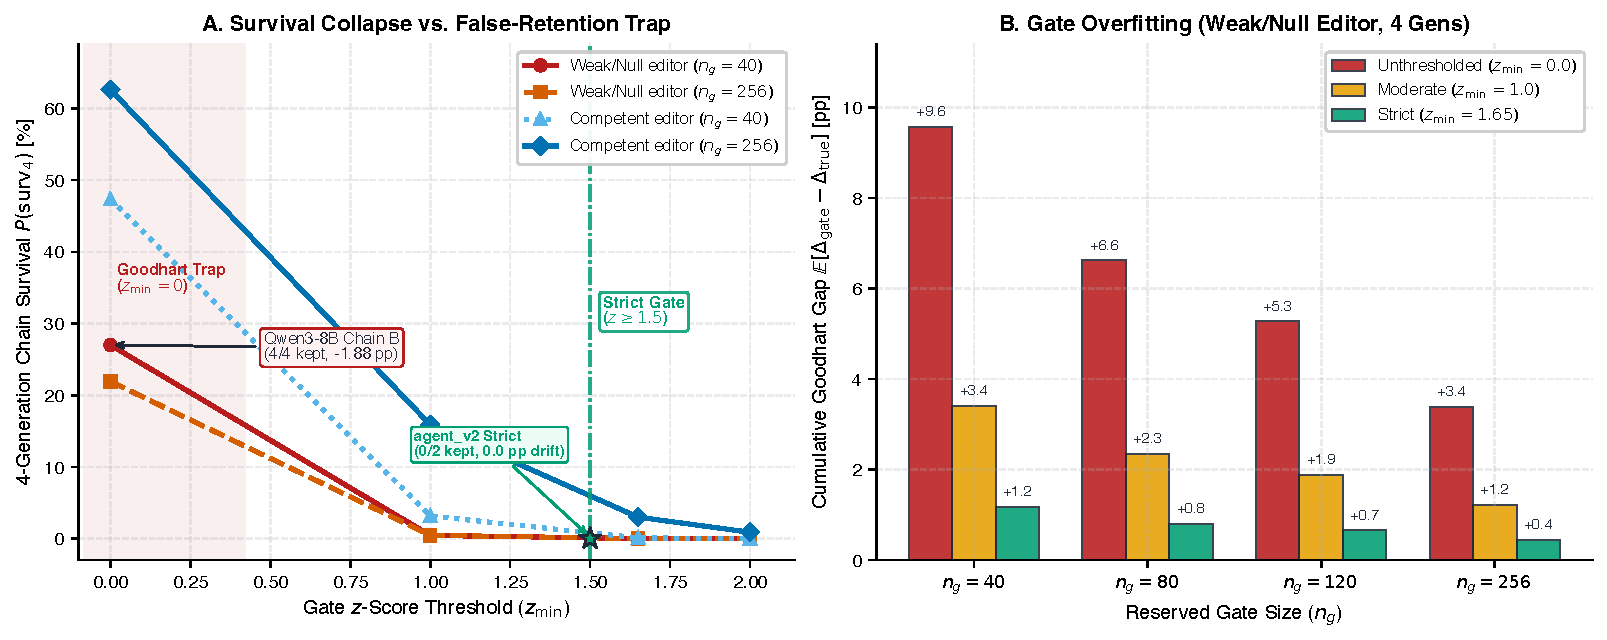
\includegraphics[width=\linewidth]{figs/fig1_gate_phase.pdf}
\caption{Retention--Drift Phase Transition (10,000 simulated 4-generation chains per cell, $A=2$, $p_{\mathrm{flip}}=0.15$). \textbf{Left:} Unthresholded $n_g=40$ gates trap weak/null editors in a 27.0\% false-survival illusion (matching Qwen3-8B Chain~B), whereas strict gates ($z_{\min}\ge 1.5$, validated live by \texttt{agent\_v2}) eliminate drift at the cost of a sharp detection-power cliff unless $n_g$ scales up. \textbf{Right:} Cumulative Goodhart gap $\mathbb{E}[\Delta_{\mathrm{gate}}-\Delta_{\mathrm{true}}]$ reaches $+9.57$\,pp at $n_g=40, z_{\min}=0$ and collapses under strict gating.}
\label{fig:gate-phase}
\end{figure}

\TableGatePhase

\subsection{The Topic-Confounding Mirage in Contrastive Activation Diagnostics}
\label{sec:mirage}

Most training-free weight-editing and activation-steering methods construct an edit direction from the mean difference between correct and incorrect practice rollouts: $v_{\mathrm{unp}} = \bar{h}_C - \bar{h}_W$ \citep{zou2023repe,sun2025thinkedit,fan2026selfrewriting}. Consider a latent decomposition of layer-$\ell$ hidden state (or MoE router logit vector) for problem $x$ and trajectory $y$:
\begin{equation}
h_\ell(x, y) \;=\; \mu_{\mathrm{topic}}(x) \;+\; s_{\mathrm{outcome}}(y) \;+\; \eta(x, y),
\end{equation}
where $\mu_{\mathrm{topic}}(x)$ captures semantic domain, difficulty, and surface features of problem $x$, while $s_{\mathrm{outcome}}(y)$ isolates within-problem reasoning divergence.

\begin{proposition}[Topic-Confounding Inflation]
\label{prop:mirage}
When $C$ and $W$ are drawn from disjoint problem subsets $\mathcal{X}_C \neq \mathcal{X}_W$ (as happens whenever single-seed practice rollouts are partitioned into $C$ vs.\ $W$), the squared norm of the expected contrastive vector satisfies
\begin{equation}
\label{eq:mirage}
\mathbb{E}\|v_{\mathrm{unp}}\|^2 \;=\; \|\mathbb{E}[\mu_{\mathrm{topic}}|\mathcal{X}_C] - \mathbb{E}[\mu_{\mathrm{topic}}|\mathcal{X}_W]\|^2 \;+\; \|s_C - s_W\|^2 \;+\; O(N^{-1}),
\end{equation}
whereas restricting strictly to \textbf{same-problem counterfactual pairs} $(x_k, y_k^{(C)}), (x_k, y_k^{(W)})$ cancels $\mu_{\mathrm{topic}}(x_k)$ identically on every pair, isolating $\|s_C - s_W\|^2$ alone.
\end{proposition}

Because topic and difficulty differences dominate high-dimensional residual streams and MoE expert routing (which specializes heavily by domain), unpaired contrasts create a massive \emph{separability mirage} ($|d| > 2.1$, router SNR $> 5$), tricking both human researchers and autonomous LLM editors into amplifying topic vectors rather than fixing reasoning errors.

\section{Training-Free Compilers and Native 4-Bit Transactional Harness}
\label{sec:methods-sys}

\subsection{Native 4-Bit Zero-Dequantization Architecture}
Legacy MLX weight-editing harnesses (\texttt{agent8b.py}) dequantized 8-bit checkpoints into dense \texttt{bfloat16} before editing. On a 128\,GB Apple M3 Max, BF16 dequantization of Qwen3-14B inflated unified memory to $77.1$\,GB plus $7.5$\,GB swap and crippled batched throughput to $31\text{--}48$\,tok/s, causing an 11-session chain to consume over 45~hours and forcing earlier roadmaps to cap model scale at $\le 9$B.

We replace dense dequantization with zero-dequantization additive wrappers directly over MLX quantized linear layers (\texttt{QuantizedLinear}) in \texttt{exp/v2/}:
\begin{itemize}[leftmargin=1.4em,itemsep=1pt,topsep=2pt]
    \item \texttt{FastLoRAWrapper}: computes $y = \mathrm{QuantizedLinear}(x) + (x A^\top) B^\top$ in FP16/BF16 with $A\in\mathbb{R}^{r\times d_{\mathrm{in}}}, B\in\mathbb{R}^{d_{\mathrm{out}}\times r}$ ($r \in \{4, 8\}$), preserving 4-bit base weights untouched in Metal memory.
    \item \texttt{RouterGateWrapper}: wraps the 256-expert MoE gate $\texttt{mlp.gate}$ as $g(x) = W_{\mathrm{gate}} x + b_{\mathrm{router}} + (x A^\top) B^\top$, enabling both direct expert-logit biasing and state-conditional low-rank router rewiring.
    \item \texttt{ResidualSteeringWrapper}: adds inference-time residual steering vectors as a matched-norm TGAS-style control \citep{nguyen2026stop}.
\end{itemize}
As shown in Table~\ref{tab:hardware} and Figure~\ref{fig:systems}A, native 4-bit execution runs the 40-layer, 256-expert \textbf{Qwen3.5-35B-A3B} at \textbf{120.8\,tok/s} ($\mathrm{bs}=64$; reaching up to $180\text{--}202.8$\,tok/s in long 3,072-token AIME batches) in only \textbf{27.3\,GB} peak unified memory---$2.8\times$ less memory and $3.5\text{--}4.5\times$ faster than legacy BF16 Qwen3-14B---while extracting full 3-layer residual, MLP, and MoE router diagnostics in $0.60$\,s.

\TableHardware

\subsection{Five Training-Free Weight Compilation Operators}
\label{sec:compilers}

For each layer $\ell$, a single-pass forward extractor captures token-level residual states $H_\ell$, pre-MLP inputs $X_\ell$, and (for MoE models) 256-expert router logits $R_\ell$ over alignment windows (\texttt{early}, \texttt{mid}, \texttt{late}, \texttt{commit}, or \texttt{all}). Given contrastive positive/negative trajectory sets $(\mathcal{P}, \mathcal{N})$---either strictly same-problem $(C, W)$ pairs, unpaired $(C, W)$ sets, or context-augmented vs.\ base rollouts---we compile five training-free operators (full derivations in Appendix~\ref{app:woodbury}):

\begin{enumerate}[leftmargin=1.4em,itemsep=2pt,topsep=2pt]
    \item \textbf{Gated DeltaNet Time-Step Bias ($\Delta b_{dt}$):} Uniformly shifts $b_{dt} \leftarrow b_{dt} + \delta$ on all 30 linear-attention layers, decreasing recurrent retention $g = \exp[-\exp(A_{\log})\,\mathrm{softplus}(a+b_{dt})]$ \citep{yang2025gateddelta,fan2026selfrewriting}.
    \item \textbf{MoE Router Contrastive Bias:} Computes Welch $t$-statistics $t_e$ across all 256 experts between $\mathcal{P}$ and $\mathcal{N}$, masks to the top-$m$ ($m=32$) experts by $|t_e|$, and installs $b_{\mathrm{router}} = \alpha\,\hat{t}_{\mathrm{top}\text{-}m}$.
    \item \textbf{State-Conditional Null-Space MoE Router LoRA:} Solves closed-form primal/Woodbury ridge regression over normalized pre-MLP states $X_\ell$ to shift router logits along $\Delta r_\ell = \bar{r}_{\mathcal{P}} - \bar{r}_{\mathcal{N}}$ specifically when encountering error states $X_{\mathcal{N}}$, while penalizing perturbations on already-correct states $X_{\mathcal{P}}$:
    \begin{equation}
    \label{eq:ridge}
    \Delta W^\star \;=\; \arg\min_{\Delta W}\; \|\Delta W X_{\mathcal{N}} - \alpha Y_{\mathrm{target}}\|_F^2 \;+\; \lambda_{\mathrm{keep}}\|\Delta W X_{\mathcal{P}}\|_F^2 \;+\; \lambda_{\mathrm{reg}}\|\Delta W\|_F^2,
    \end{equation}
    truncated via SVD to rank $r=8$. This extends AlphaEdit's null-space preservation \citep{fang2025alphaedit} to sparse MoE routing without gradients.
    \item \textbf{Woodbury Null-Space MLP LoRA:} Solves Eq.~\eqref{eq:ridge} directly on MLP/shared-expert \texttt{down\_proj} inputs ($d_{\mathrm{in}}\le 17{,}408$) using the Woodbury matrix identity in token space ($O(N^3)$ instead of $O(d_{\mathrm{in}}^3)$), targeting residual shift $\bar{h}_{\mathcal{P}} - \bar{h}_{\mathcal{N}}$ at rank $r=4$.
    \item \textbf{Training-Free Context-to-Weight Internalization:} Runs identical practice problems twice---once with base prompt and once with a concise/analytical system instruction---then compiles the exact hidden-state or MoE router shift $\Delta_{\mathrm{ctx}} = h(\text{prompted}) - h(\text{base})$ permanently into MLP LoRA or MoE Router LoRA via Eq.~\eqref{eq:ridge}, allowing prompt-free inference at test time (analogous to gradient-free BaseRSI \citealt{zhang2026basersi} and Halt Vector \citealt{jayabahu2026halt}).
\end{enumerate}

\subsection{Transactional Autonomous Harness (\texttt{agent\_v2})}
Forensic inspection of our legacy BF16 chains (\S\ref{sec:expc}) revealed severe harness fragility: in the Qwen3-14B chain, \LegacyFourteenErr{} of autonomous turns crashed due to banned Python builtins (\texttt{type}, \texttt{hasattr}, \texttt{.format}), mutable global tool bindings (one session overwrote its own readout function with a dictionary and failed 8 consecutive turns), and non-transactional weight edits (an aborted turn left a permanent $+0.1I$ ghost mutation on \texttt{layers.0.self\_attn.o\_proj}).

Our \texttt{agent\_v2.py} harness resolves all four failure modes: (i) a read-only \texttt{tools.*} namespace that raises \texttt{AttributeError} on assignment; (ii) safe introspection builtins (\texttt{type}, \texttt{isinstance}, \texttt{hasattr}) plus high-level diagnostic/compiler APIs; (iii) \textbf{atomic per-turn transactions} that roll back any staged weight edits raised prior to an exception; and (iv) disk-cached base evaluations coupled with an automated \textbf{strict statistical gate} ($n_g=64$, requiring $\Delta \ge +2$\,pp, $z \ge 1.5$, one-sided $p \le 0.07$), contrasted directly against an unthresholded loose-gate ablation ($n_g=40, \Delta > 0$).

\section{Experimental Protocol and Self-Calibrated RL Stopping}
\label{sec:calib}

We evaluate seven models across six benchmarks: \textbf{MATH-500} \citep{hendrycks2021math,lightman2023verify}, temporally split \textbf{AIME} (2010--2018 practice, 2019--2021 gate, 2022--2025 held-out), \textbf{OlympiadBench-Physics} \citep{he2024olympiadbench}, \textbf{MMLU-Pro STEM} \citep{wang2024mmlupro}, \textbf{SuperGPQA-Hard Science} \citep{du2025supergpqa}, and \textbf{GPQA-Diamond} \citep{rein2023gpqa}. All held-out comparisons use problem-paired two-seed averages ($s\in\{1000,2000\}$) with paired $t$-tests, exact sign tests, problem-level percentile bootstraps, and matched-norm random controls.

\paragraph{Finding 1: Self-Calibrated RL Stopping Masks Reasoning Errors.}
Before testing reasoning edits, we calibrated conditional accuracy given finish ($\mathrm{acc}|\mathrm{fin}$) across models and benchmarks (Figure~\ref{fig:regime}B). Across standard reasoning setups, modern RL-trained checkpoints exhibit extreme self-calibrated stopping: whenever uncertain, they continue generating until truncation rather than emitting a wrong answer. Specifically, $\mathrm{acc}|\mathrm{fin}$ reaches \textbf{100.0\%} on MATH-500 (Qwen3.5-4B at 16k), \textbf{99.8\%} on MATH-500 (Qwen3-14B at 4k), \textbf{99.4\%} on MMLU-Pro STEM across 256 rollouts (Qwen3.5-9B \texttt{nothink} at 2k: only $W=1$ finished-wrong answer in 256!), \textbf{100.0\%} on AIME 2010--2018, and \textbf{90.9\%} on AIME 2024--2025 (Qwen3.5-35B-A3B \texttt{nothink} at 3k). Because $W$ approaches zero, standard benchmarks physically cannot measure $W\!\to\!C$ improvement.

To break completion saturation and isolate genuine reasoning errors, we introduce a \textbf{Brief-CoT protocol} ($\mathrm{cap}=768$, instructing a 3--5 sentence justification under 200 words) on graduate-level SuperGPQA-Hard and GPQA-Diamond. This immediately unlocks abundant finished-wrong answers: SuperGPQA-Hard yields $\mathrm{acc}|\mathrm{fin}=40\text{--}47\%$ ($W=22\text{--}31\%$, $\mathrm{pass@1}=19.9\% \to \mathrm{pass@4}=31.3\%$) and GPQA-Diamond yields $\mathrm{acc}|\mathrm{fin}=74\text{--}86\%$ ($\mathrm{pass@1}=65.3\% \to \mathrm{pass@5}=82.8\%$), supplying strictly same-problem $(C, W)$ counterfactual pairs for mechanistic editing.

\section{Experimental Results}
\label{sec:results}

\subsection{Budget Dependence and Thinking-Mode Failure Boundary (Phase 1 \& Exp A)}
\label{sec:expa}

Figure~\ref{fig:regime}A summarizes both our cross-checkpoint replication of \citet{fan2026selfrewriting}'s session-8 edit ($\Delta b_{dt}=+0.5$) on Qwen3.5-4B (MATH-500, $n=400\times 2$) and its sharp failure boundary on Qwen3.5-35B-A3B (Experiment~A, AIME 2024--2025, $n=32$).

On Qwen3.5-4B at the pre-specified 16,384-token cap, $\Delta b_{dt}=+0.5$ raises two-seed accuracy from $69.125\%$ to $74.000\%$ ($\Delta = +4.875$\,pp, 95\% CI $[+1.20,+8.55]$, paired $p=0.00947$), far above a matched-magnitude random-sign control ($-8.50$\,pp vs.\ base, $p=0.0011$). However, Proposition~\ref{prop:decomp} exposes its exact mechanism: across 800 paired evaluations, \textbf{196 of 197 binary score changes are $T\!\leftrightarrow\!C$ transitions} ($N_{T,C}=118, N_{C,T}=78, N_{W,C}=0, N_{C,W}=1$), yielding $\Delta_{\mathrm{comp}}=+5.00$\,pp and $\Delta_{\mathrm{reas}}=-0.125$\,pp. At tight budgets (4,096 tokens), the weight edit yields only $+0.50$\,pp ($p=0.74$), whereas a one-sentence concision prompt achieves $+13.13$\,pp ($p=7.4\times 10^{-11}$).

In \textbf{Experiment~A}, we test whether $\Delta b_{dt}$ can rescue Qwen3.5-35B-A3B in full thinking mode on hard competition math (AIME 2024--2025, cap 4,096) across a six-point dose sweep $\Delta b_{dt} \in \{+0.3, +0.5, +0.8, +1.2, +1.6\}$ plus random-sign $\pm 0.8$ and concision prompting. \textbf{Every single one of the 8 arms scores 0.0\% (32/32 truncated, 0/32 closed \texttt{</think>}).} Transcript inspection reveals compulsive post-solution re-verification (e.g., computing the exact answer early and spending the remaining 3,500 tokens doubting it); increasing $\Delta b_{dt}$ to $+1.6$ triggers literal token repetition ($3.1\%$ looping) before ever inducing termination. Thus, Gated DeltaNet decay shifts modulate \emph{marginal} stopping probability only when trajectories are already near completion, and fail completely under strong RL-induced over-verification.

\begin{figure}[tbp]
\centering
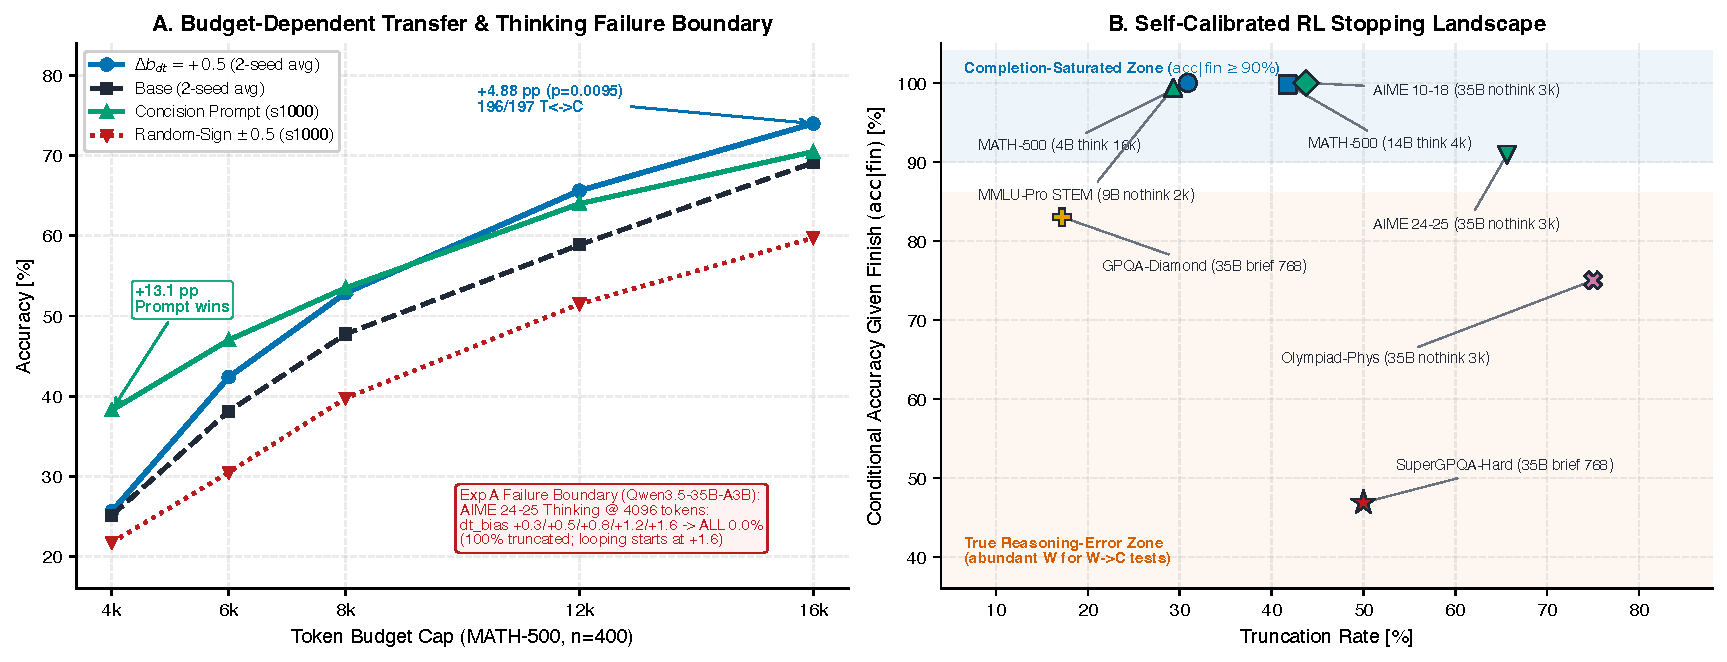
\includegraphics[width=\linewidth]{figs/fig4_regime_boundaries.pdf}
\caption{\textbf{A.} Cross-checkpoint replication of $\Delta b_{dt}=+0.5$ on Qwen3.5-4B (MATH-500, $n=400$) showing strong budget dependence (concision prompt dominates at 4k; edit wins at 16k purely via 196/197 $T\!\leftrightarrow\!C$ flips) alongside Experiment~A's complete failure boundary on AIME 24--25 thinking mode. \textbf{B.} Self-Calibrated RL Stopping landscape across models and benchmarks: standard regimes saturate $\mathrm{acc}|\mathrm{fin}\ge 90\%$, while Brief-CoT unlocks true $W$ errors.}
\label{fig:regime}
\end{figure}

\subsection{The Topic-Confounding Mirage and Subspace Orthogonality (Pilot 1, Exp B \& Exp D)}
\label{sec:exp-mirage}

In \textbf{Pilot~1} (Qwen3.5-35B-A3B, SuperGPQA-Hard \texttt{nothink}, cap 2,048, 14 edited arms), unpaired $C$-vs-$W$ diagnostics displayed dramatic apparent separability across all 40 MoE layers---peaking at layer-20 router $\mathrm{SNR}=6.15$ ($\max|t|=7.98$) and layer-38 residual $|d|=1.60$---yet installing those directions \emph{reduced} held-out accuracy ($-4.69$\,pp and $-3.12$\,pp). Simultaneously, measuring cosine alignment between $(C\text{-}W)$ and $(C\text{-}T)$ contrasts across all 19 scanned layers revealed near-orthogonality: mean $|\cos(v_{C\text{-}W}, v_{C\text{-}T})| = \OrthResCos$ in residual space and $\OrthRtrCos$ in 256-expert MoE router space (Figure~\ref{fig:mirage}C).

To test Proposition~\ref{prop:mirage} directly across two independent benchmarks, we mined strictly same-problem $(C, W)$ pairs and compared them against size-matched, strictly disjoint-problem $(C, W)$ pairs across all 40 MoE layers (Figure~\ref{fig:mirage}A--B):
\begin{itemize}[leftmargin=1.4em,itemsep=1pt,topsep=2pt]
    \item \textbf{SuperGPQA-Hard (Exp~B, 512 rollouts, $N=12$ matched pairs):} Mean residual $|{\rm Cohen's}\ d|$ plunges by $\mathbf{\MirageSGRatioD}$ ($\MirageSGUnpD \to \MirageSGSameD$, \textbf{\MirageSGConfoundD{}} topic confounding), and mean 256-expert MoE router SNR plunges by $\mathbf{\MirageSGRatioSNR}$ ($\MirageSGUnpSNR \to \MirageSGSameSNR$, \textbf{\MirageSGConfoundSNR{}} confounding).
    \item \textbf{GPQA-Diamond Replication (Exp~D, 320 rollouts, $22$ same-problem pairs, $N=19$ matched disjoint pairs):} The exact same collapse replicates independently---mean residual $|d|$ plunges by $\mathbf{\MirageGPQARatioD}$ ($\MirageGPQAUnpD \to \MirageGPQASameD$, \textbf{72.7\%} topic confounding), and mean 256-expert MoE router SNR plunges by $\mathbf{\MirageGPQARatioSNR}$ ($\MirageGPQAUnpSNR \to \MirageGPQASameSNR$, \textbf{77.3\%} confounding).
\end{itemize}
Across both benchmarks, roughly three-quarters of the apparent activation and expert-routing signal separating correct from wrong rollouts is a topic-confounding artifact.

\begin{figure}[tbp]
\centering
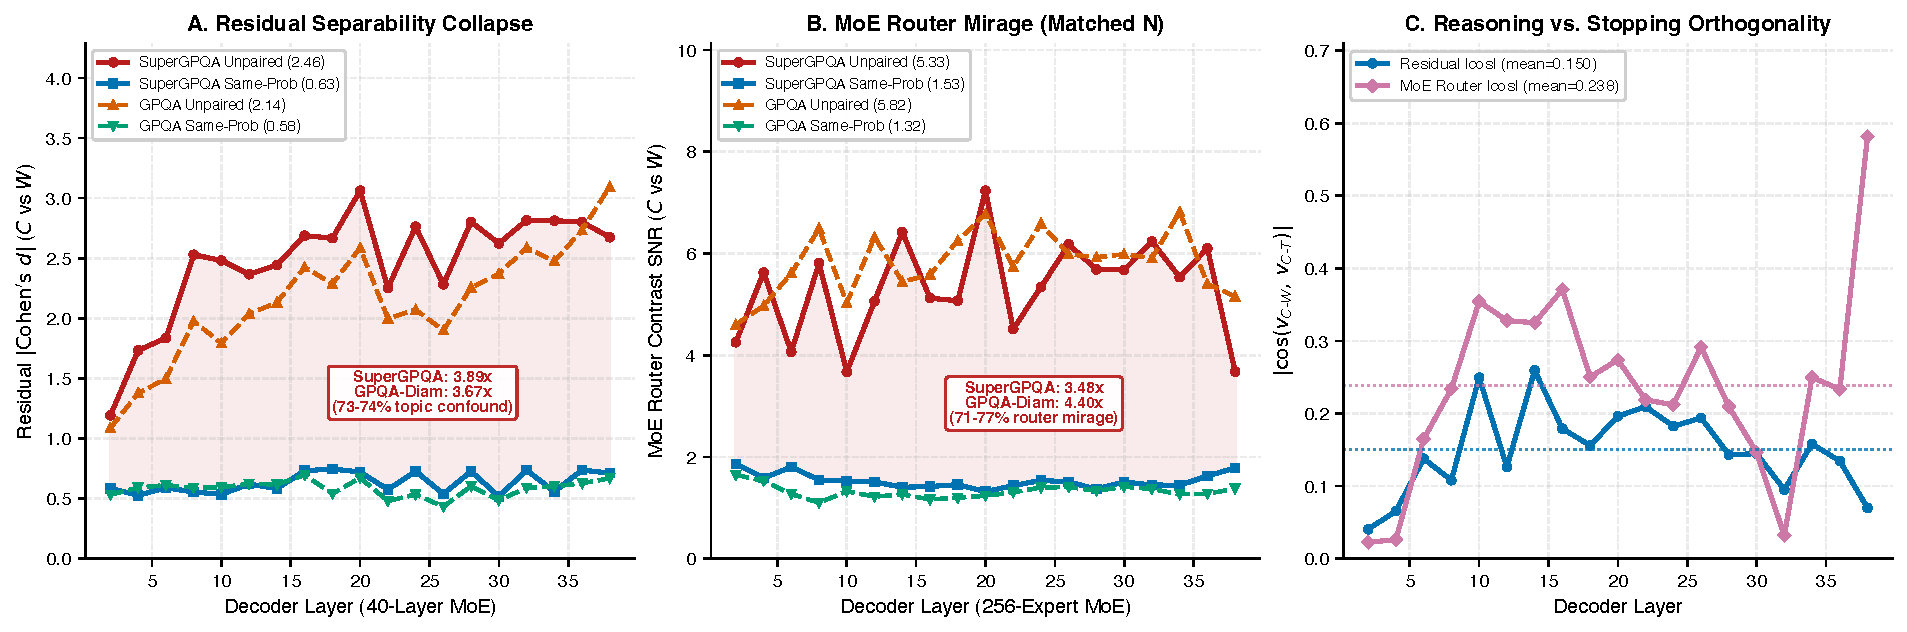
\includegraphics[width=\linewidth]{figs/fig2_mirage_geometry.pdf}
\caption{Geometric proof of the Topic-Confounding Mirage across 40 MoE layers of Qwen3.5-35B-A3B on two independent benchmarks (SuperGPQA-Hard and GPQA-Diamond, matched $N$). \textbf{A.} Residual $|\mathrm{Cohen's}\ d|$ collapses $\MirageSGRatioD$ on SuperGPQA-Hard and $\MirageGPQARatioD$ on GPQA-Diamond when problem identity is held constant. \textbf{B.} 256-expert MoE router SNR collapses $\MirageSGRatioSNR$ and $\MirageGPQARatioSNR$. \textbf{C.} Reasoning ($C\text{-}W$) and stopping ($C\text{-}T$) directions are nearly orthogonal ($|\cos|=\OrthResCos$ residual, $\OrthRtrCos$ router).}
\label{fig:mirage}
\end{figure}

\subsection{Universal Completion--Accuracy Tradeoff and Zero-Shot Transfer (Exp B)}
\label{sec:expb}

Table~\ref{tab:expb-main} and Figure~\ref{fig:tradeoff}A present the complete Experiment~B evaluation on held-out SuperGPQA-Hard ($128$ problems $\times\, 2$ seeds $= 256$ paired evaluations per arm, 2,816 test rollouts total). Two striking laws emerge:

\begin{enumerate}[leftmargin=1.4em,itemsep=2pt,topsep=2pt]
    \item \textbf{9/9 Completion-Positive, Reasoning-Negative Sign Pattern:} Every single weight and activation intervention---Gated DeltaNet $\Delta b_{dt}=+0.5$, same-problem MoE router bias, same-problem null-space router LoRA, unpaired-mirage router bias, context-internalized MoE router, random router control, same-problem null-space MLP LoRA, context-internalized MLP LoRA, and TGAS-style residual steering---exhibits $\Delta_{\mathrm{comp}} > 0$ ($+0.78$ to $+4.69$\,pp) paired with $\Delta_{\mathrm{reas}} < 0$ ($-0.39$ to $-1.56$\,pp). Under a symmetric null for $\Delta_{\mathrm{reas}}$, observing 9/9 negative signs has probability $2^{-9} = 0.00195$. Conversely, a verification prompt (\texttt{prompt\_verify\_brief}) lengthens reasoning ($+102$\,tokens), slashing accuracy by $-13.28$\,pp ($p=1.15\times 10^{-5}$, $\Delta_{\mathrm{comp}}=-13.67$\,pp) while nudging $\Delta_{\mathrm{reas}}=+0.39$\,pp.
    \item \textbf{Acute Token-Compression vs.\ Accuracy Tradeoff on Zero-Shot Transfer:} Evaluating SuperGPQA-compiled edits zero-shot on GPQA-Diamond ($n=128$, Table~\ref{tab:expb-gpqa-transfer}, Figure~\ref{fig:tradeoff}B) crystallizes the tradeoff. \textbf{Context-to-weight MoE Router internalization} permanently compresses output length by \textbf{\GPQATokCut{}} ($438.6 \to 229.9$ tokens, with zero prompt overhead), generating a massive completion surge ($\Delta_{\mathrm{comp}}=+8.59$\,pp, $14\,T\!\to\!C$ vs.\ $3\,C\!\to\!T$), yet simultaneously losing $\Delta_{\mathrm{reas}}=-6.25$\,pp ($10\,W\!\to\!C$ vs.\ $18\,C\!\to\!W$) for a net $+2.34$\,pp gain. Meanwhile, $\Delta b_{dt}=+0.5$ transfers $+4.69$\,pp cleanly via pure completion ($+4.69$\,pp $T\!\to\!C$, $0.00$\,pp $W\!\to\!C$), while context-internalized MLP LoRA preserves length ($-5.5\%$ tokens) and is the lone arm with nominal positive $\Delta_{\mathrm{reas}}=+3.12$\,pp ($6\,W\!\to\!C$ vs.\ $2\,C\!\to\!W$, $p=0.29$).
\end{enumerate}

\begin{figure}[tbp]
\centering
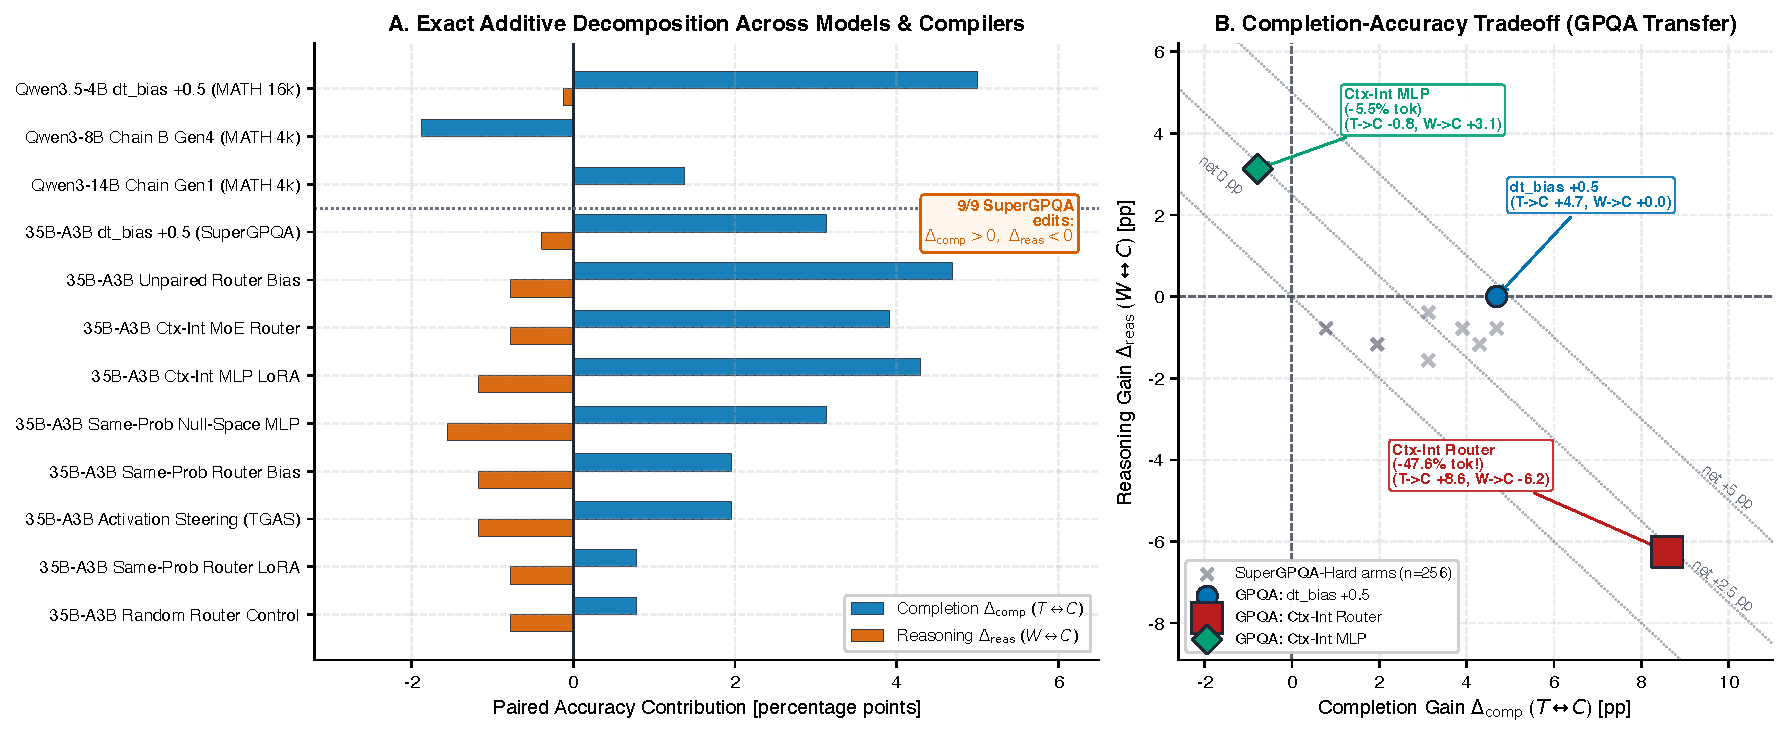
\includegraphics[width=\linewidth]{figs/fig3_universal_tradeoff.pdf}
\caption{\textbf{A.} Exact additive decomposition $\Delta = \Delta_{\mathrm{comp}} + \Delta_{\mathrm{reas}}$ across Qwen3.5-4B, Qwen3-8B/14B chains, and all 9 training-free compilers/controls in Experiment~B: every single SuperGPQA-Hard edit (9/9) raises completion at the expense of finished-answer accuracy. \textbf{B.} Zero-shot GPQA-Diamond transfer (marker area $\propto$ token reduction) exposes the sharp Completion--Accuracy Pareto frontier, with MoE Router context internalization cutting tokens by \GPQATokCut{} ($+8.59$\,pp $T\!\to\!C$, $-6.25$\,pp $W\!\to\!C$).}
\label{fig:tradeoff}
\end{figure}

\TableExpBMain
\TableExpBGPQATransfer

\subsection{GPQA-Diamond In-Domain Replication and Cross-Domain OOD Harm (Exp D)}
\label{sec:expd}

Experiment~D tests two decisive boundary conditions: (i) whether same-problem $(C, W)$ compilation succeeds in-domain on high-latent-gap GPQA-Diamond ($134\times 2=268$ strictly unseen evaluations per arm, Table~\ref{tab:expd-gpqa}, Figure~\ref{fig:crossdomain}A), and (ii) whether Fan et al.'s $\Delta b_{dt}$ edit transfers across domains from competition mathematics (AIME 2022--2025, $n=64\times 2$) to zero-shot out-of-domain physics (OlympiadBench-Physics, $n=64\times 2$, Table~\ref{tab:expd-cross}, Figure~\ref{fig:crossdomain}B).

\begin{enumerate}[leftmargin=1.4em,itemsep=2pt,topsep=2pt]
    \item \textbf{6/6 GPQA-Diamond Replication (15/15 Combined):} Every single GPQA-Diamond weight and steering arm---$\Delta b_{dt}=+0.5$, same-problem MoE router bias, same-problem router null-space LoRA, same-problem MLP null-space LoRA, random router control, and TGAS activation steering---again yields $\Delta_{\mathrm{comp}} > 0$ ($+0.37$ to $+3.36$\,pp) paired with $\Delta_{\mathrm{reas}} \le 0$ ($-1.12$ to $0.00$\,pp). Pooling Experiment~B (9/9) and Experiment~D Part~1 (6/6), \textbf{15 out of 15} multi-seed Brief-CoT interventions across both graduate-science benchmarks produce $\Delta_{\mathrm{comp}}>0$ (two-sided sign test $p=6.1\times 10^{-5}$) and \textbf{0 out of 15} produce positive $\Delta_{\mathrm{reas}}$. Even matched-norm random router bias ($+1.12$\,pp) outperforms all three targeted same-problem weight compilers ($-0.75$ to $+0.75$\,pp).
    \item \textbf{Statistically Significant OOD Harm of $\Delta b_{dt}=+0.5$ on OlympiadBench-Physics:} Under \texttt{nothink} (cap 3,072), a one-sentence concision prompt achieves a statistically significant \textbf{$+7.81$\,pp gain on AIME 2022--2025} ($28.12\%\to 35.94\%$, 95\% CI $[+1.56,+14.06]$, $p=0.017$, $\Delta_{\mathrm{comp}}=+7.03$\,pp) and $+3.91$\,pp on OlympiadBench-Physics ($20.31\%\to 24.22\%$). By stark contrast, \textbf{$\Delta b_{dt}=+0.5$ fails on AIME ($-0.78$\,pp, $p=0.784$) and causes a statistically significant $-7.03$\,pp accuracy collapse on out-of-domain OlympiadBench-Physics} ($20.31\%\to 13.28\%$, 95\% CI $[-13.28,-1.56]$, $p=0.019$, $\Delta_{\mathrm{comp}}=-6.25$\,pp, $\Delta_{\mathrm{reas}}=-0.78$\,pp)---trailing concision prompting by $10.94$\,pp! Higher dose $\Delta b_{dt}=+0.8$ also drops AIME by $-5.47$\,pp ($p=0.163$). Thus, Gated DeltaNet \texttt{dt\_bias} edits are not general reasoning enhancers: they are brittle, domain- and mode-sensitive recurrent decay perturbations that actively harm out-of-domain scientific derivation.
\end{enumerate}

\begin{figure}[tbp]
\centering
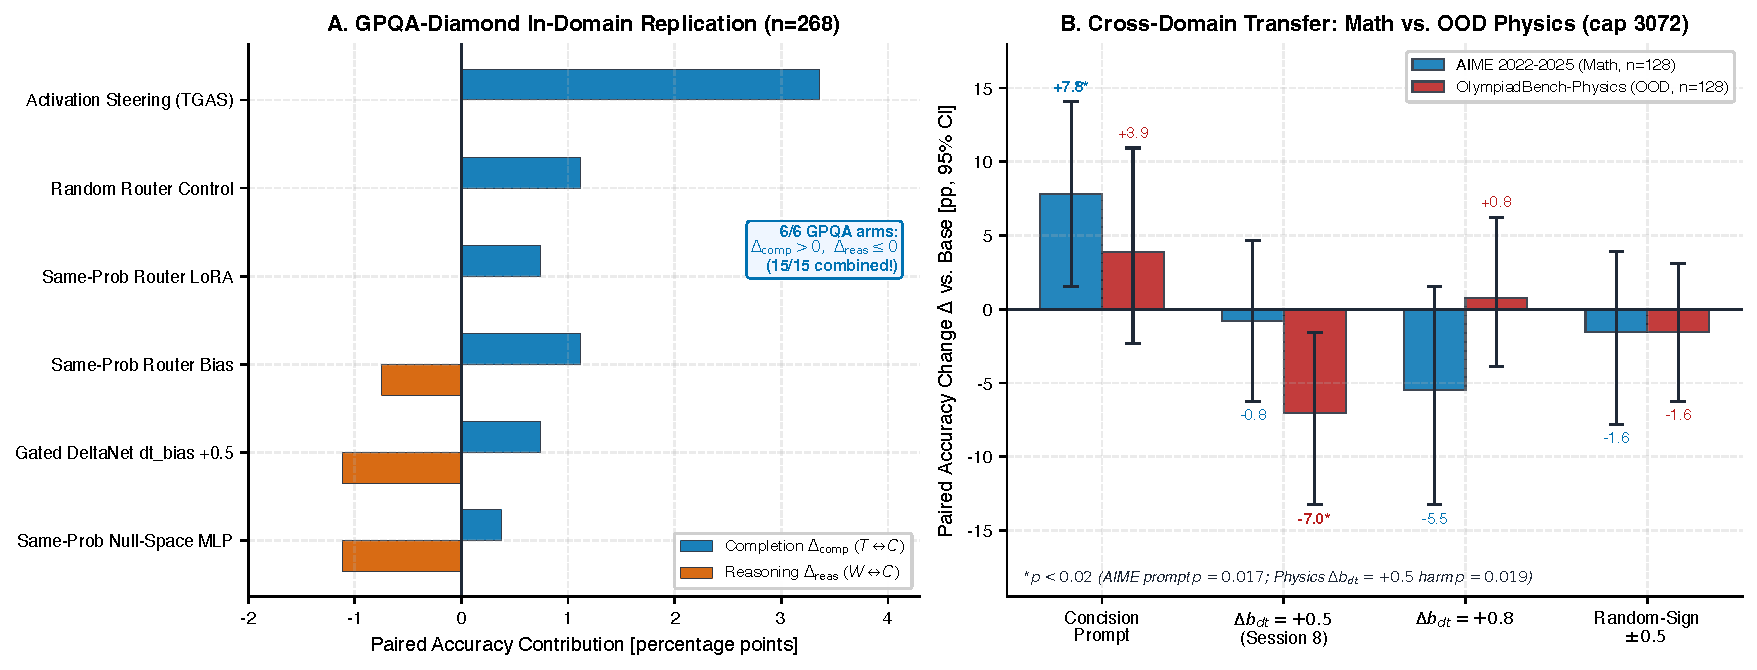
\includegraphics[width=\linewidth]{figs/fig6_crossdomain_ood.pdf}
\caption{Experiment~D results on Qwen3.5-35B-A3B. \textbf{A.} In-domain GPQA-Diamond same-problem compilation ($n=268$): 6/6 weight and steering arms yield $\Delta_{\mathrm{comp}}>0$ and $\Delta_{\mathrm{reas}}\le 0$ (15/15 combined with SuperGPQA-Hard, $p=6.1\times 10^{-5}$). \textbf{B.} Cross-domain transfer at cap 3,072 (\texttt{nothink}): concision prompting gains $+7.81$\,pp on AIME 22--25 ($p=0.017$) and $+3.91$\,pp on Physics, while Fan et al.'s $\Delta b_{dt}=+0.5$ induces a statistically significant $-7.03$\,pp degradation on out-of-domain OlympiadBench-Physics ($p=0.019$).}
\label{fig:crossdomain}
\end{figure}

\TableExpDGPQA
\TableExpDCrossDomain

\subsection{Autonomous Recursive Chains: Legacy Fragility vs.\ Transactional \texttt{agent\_v2} (Phase 2 \& Exp C)}
\label{sec:expc}

Table~\ref{tab:expc-chains} and Figure~\ref{fig:systems}B compare our two legacy BF16 chains (\texttt{agent8b.py}) against native 4-bit transactional \texttt{agent\_v2} under Strict ($n_g=64, z\ge 1.5$) vs.\ Loose ($n_g=40, \Delta>0$) gating:

\begin{itemize}[leftmargin=1.4em,itemsep=2pt,topsep=2pt]
    \item \textbf{Qwen3-8B Chain~B (Legacy Loose Gate):} Retained an edit in \textbf{4/4 generations} despite never inspecting a single problem or failed answer ($0/7$ diagnostic sessions) and applying only uniform or random directions. Confirming on $\pm 1\text{--}2$ problem gate flips (including a negative $-5.0$\,pp gate check in generation~2), generation~4 landed at $\mathbf{-1.88\,\text{pp}}$ held-out ($[-4.14,+0.39], p=0.104$, $\Delta_{\mathrm{reas}}=0.00$\,pp)---a textbook empirical instance of Theorem~\ref{thm:phase}'s Goodhart Trap.
    \item \textbf{Qwen3-14B Chain (Legacy Loose Gate):} Suffered a \textbf{\LegacyFourteenErr{}} turn crash rate and a ghost $+0.1I$ mutation on \texttt{L0.o\_proj} from a crashed turn. Generation~1 confirmed a massive $+0.15I\text{--}+0.40I$ identity shift after a $+10$\,pp ($5/1$) gate swing, while generation~2 withdrew a $0.14\text{--}0.34\%$ perturbation after an equal and opposite $-10$\,pp ($1/5$) swing---directly proving that $n_g=40$ noise dwarfs edit signal. Held-out primary result: $+1.38$\,pp ($[-0.81,+3.56], p=0.216$), below the unedited model's $+1.75$\,pp reseed noise, with $W\!\to\!C = 0/800$ and $C\!\to\!W = 0/800$.
    \item \textbf{Qwen3.5-35B-A3B (\texttt{agent\_v2} Strict \& Loose Gate, Exp~C):} Under our transactional native 4-bit harness, autonomous session quality transformed qualitatively. Turn generation took $3.5\text{--}14.8$\,s (vs.\ $4\text{--}12$\,min on BF16 14B); diagnostic engagement jumped to \textbf{100\%} ($4/4$ sessions across both runs); turn error rate fell from \textbf{42.2\%} (14B) to \textbf{17.6\%} ($3/17$ per run, zero sandbox/namespace crashes, with every argument/budget error atomically rolled back and \textbf{zero ghost edits}). In Attempt~1, Qwen3.5-35B-A3B read its own physics mistakes, scanned 40 MoE layers, compiled a 9-layer Woodbury MLP LoRA ($L30\text{--}38$), observed $+10\text{--}13.3$\,pp on practice subsets, and submitted; the Strict Gate ($n_g=64$) caught $-4.69$\,pp ($z=-0.90, p=0.887$) and atomically rejected it, while the Loose Gate ($n_g=40$) recorded $0.00$\,pp ($1/1$) and likewise rejected it. In Attempt~2, the model compiled a 9-layer MoE Router Bias ($L30\text{--}38$, $+15$\,pp on 20 practice problems), tested stacking a 10-layer mid-network Null-Space LoRA ($L15\text{--}24$), observed cancellation back to $0.0$\,pp, and \textbf{autonomously invoked \texttt{tools.rollback()}} rather than blindly committing noise. Both chains terminated cleanly at generation~1 with \textbf{$0.00$\,pp held-out drift}, demonstrating that even when a 35B MoE conducts genuinely disciplined autonomous diagnosis and compilation, training-free updates hit the completion-only ceiling on hard graduate science.
\end{itemize}

\begin{figure}[tbp]
\centering
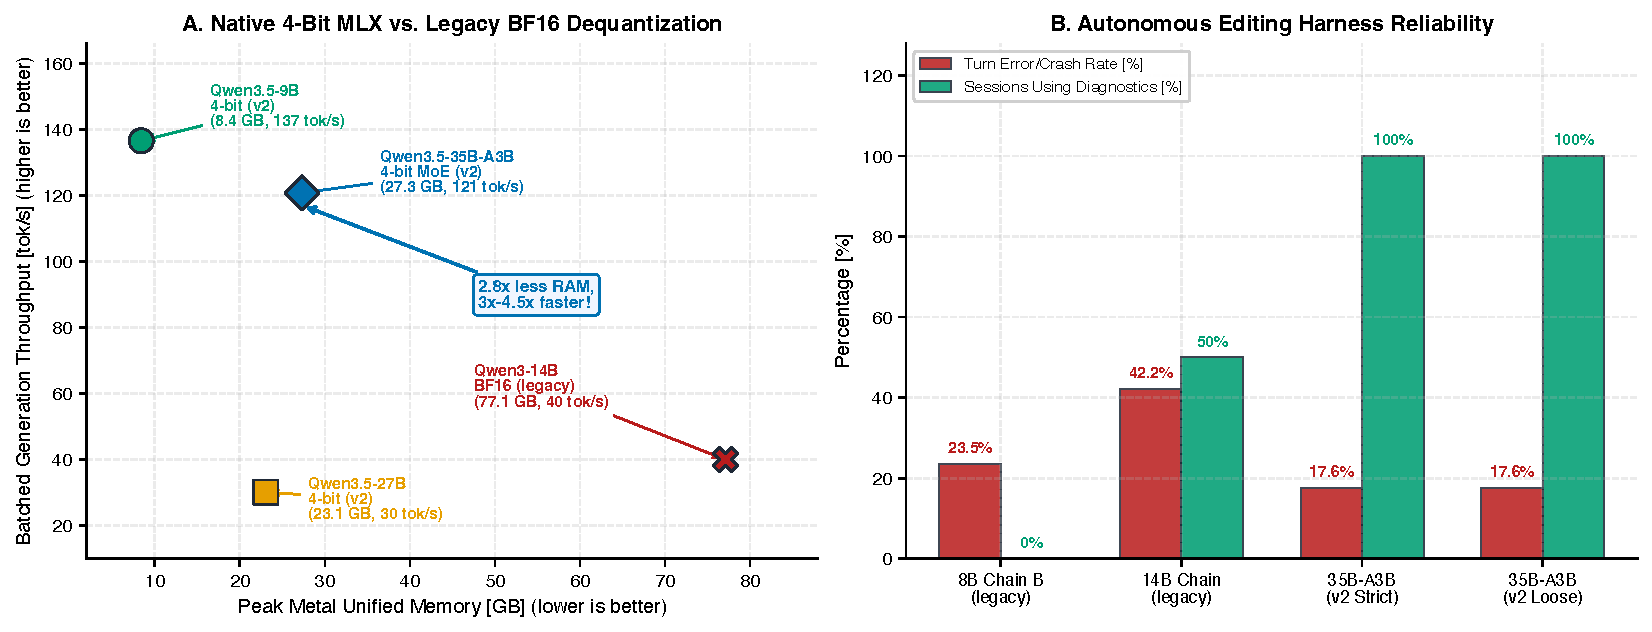
\includegraphics[width=\linewidth]{figs/fig5_systems_harness.pdf}
\caption{\textbf{A.} Hardware efficiency leap on Apple M3 Max (128\,GB): native 4-bit MLX wrappers run 35B-A3B MoE in 27.3\,GB at 120.8\,tok/s---2.8$\times$ less RAM and 3.5--4.5$\times$ faster than BF16-dequantized Qwen3-14B. \textbf{B.} Autonomous harness reliability comparing legacy \texttt{agent8b.py} turn crash rates (\LegacyEightErr{} on 8B; \LegacyFourteenErr{} on 14B) and diagnostic engagement against transactional \texttt{agent\_v2} ($17.6\%$ error rate, $100\%$ diagnostic usage, zero ghost edits).}
\label{fig:systems}
\end{figure}

\TableExpCChains

\section{Discussion: Why Training-Free Edits Hit a Completion-Only Ceiling}
\label{sec:discussion}

Synthesizing our geometric, statistical, and empirical evidence reveals a deep mechanistic asymmetry between \emph{controlling reasoning length} and \emph{improving reasoning accuracy}:

\paragraph{Low-rank global stopping vs.\ high-rank instance-specific reasoning.}
Termination and verbosity are governed by a low-dimensional, problem-invariant control manifold: adding $+0.5$ to \texttt{dt\_bias} uniformly attenuates recurrent memory across all tokens, and context-internalized MoE router shifts globally bias token routing toward shorter derivations (\GPQATokCut{} token reduction on GPQA-Diamond). Because this manifold is shared across problems, a single rank-1 to rank-8 training-free weight perturbation acts robustly on completion ($\Delta_{\mathrm{comp}} > 0$ across 15/15 Brief-CoT arms), yet remains fragile across domains (reversing to $-7.03$\,pp, $p=0.019$, on out-of-domain OlympiadBench-Physics). By contrast, once topic confounding is stripped away via same-problem $(C, W)$ counterfactuals, genuine reasoning errors ($W$) do \emph{not} share a low-rank global direction: residual separability collapses $\MirageSGRatioD\text{--}\MirageGPQARatioD$ to $|d|\approx 0.58\text{--}0.63$, and MoE router SNR collapses $\MirageSGRatioSNR\text{--}\MirageGPQARatioSNR$ to $1.32\text{--}1.53$. Fixing an integral substitution in one physics derivation requires an orthogonal parameter update to fixing a stereochemistry error in another; biasing weights along an average direction therefore introduces interference that caps $\Delta_{\mathrm{reas}} \le 0$ across all 15 Brief-CoT edits.

\paragraph{Reframing training-free weight editing for RSI.}
Our findings do not imply that training-free weight self-rewriting is useless---rather, they delineate its exact operational boundary. First, training-free internalization of concision and anti-loop priors is a genuinely valuable \emph{inference-efficiency compiler}: permanently cutting GPQA-Diamond token usage nearly in half (\GPQATokCut{}) in weights without prompt overhead yields immediate latency and compute savings when operating near a tight budget ceiling. Second, genuine capability compounding ($\Delta_{\mathrm{reas}} > 0$ across multiple generations without OOD regression) faces three hard prerequisites: (i) \textbf{verifier-backed gradient or high-rank episodic updates} (e.g., SEAL-style self-generated fine-tuning \citealt{zweiger2025selfadapting}) capable of resolving instance-specific reasoning errors rather than global stopping bias; (ii) \textbf{statistically powered, multi-domain gates} ($n_g \ge 256$, $z_{\min} \ge 1.65$, plus OOD guardrails) paired with exact $\Delta_{\mathrm{comp}} / \Delta_{\mathrm{reas}}$ monitoring to prevent Goodhart drift and OOD collapse; and (iii) \textbf{transactional editing harnesses} (\texttt{agent\_v2}) that isolate scientific failure from sandbox crashes and ghost parameter corruption.

\section{Limitations and Reproducibility}
\label{sec:limitations}

\paragraph{Limitations.}
All experiments run on open-weight Qwen3 and Qwen3.5 checkpoints (1.7B--35B-A3B) on a single 128\,GB Apple M3 Max workstation; frontier-scale models ($>100$B parameters) or alternative post-training recipes could exhibit higher within-problem diagnostic rank or stronger autonomous self-coding. Our Brief-CoT protocol successfully unlocked finished-wrong responses ($W$) at low latency, but tighter caps necessarily emphasize the completion--accuracy frontier compared to 32k+ unconstrained budgets. Finally, because pretraining exposure of public benchmarks is unknown, our ``held-out'' designation strictly reflects zero access by the editing algorithms or autonomous agent.

\paragraph{Reproducibility and Verification.}
Every experiment, cached rollout pickle, diagnostic extraction, and statistical test is deterministically seeded and logged in the \texttt{bootstrap-rsi} codebase (\texttt{exp/v2/}). A single standalone script, \texttt{exp/v2/verify\_all\_numbers.py}, recomputes every statistic, verifies Proposition~\ref{prop:decomp}'s exact identity ($\Delta = \Delta_{\mathrm{comp}} + \Delta_{\mathrm{reas}}$) to $10^{-9}$ tolerance across all arms, and programmatically emits \texttt{tables\_auto.tex} and all six figures (\texttt{make\_paper\_figs.py}) with zero manual transcription.

\paragraph{AI Assistance Statement.}
Under the author's direction, oversight, and verification, AI coding assistants helped engineer the evaluation harnesses, execute automated experiment suites, verify statistical scripts, and draft portions of the manuscript. The author bears full responsibility for all scientific claims, analyses, and released code.

\clearpage
\bibliographystyle{plainnat}
\bibliography{refs}

\clearpage
\appendix

\section{Analytical Proofs}
\label{app:proofs}

\subsection{Proof of Theorem~\ref{thm:phase} (Retention--Drift Phase Transition)}
Let $\delta_{\mathrm{true}} \sim \mathcal{N}(\mu, \sigma^2)$ and independent finite-sample gate noise $\varepsilon_g \sim \mathcal{N}(0, \mathrm{SE}_g^2)$ with $\mathrm{SE}_g = \sqrt{p_{\mathrm{flip}}/n_g}$. Then $\hat{\delta}_{\mathrm{gate}} = \delta_{\mathrm{true}} + \varepsilon_g \sim \mathcal{N}(\mu, v_g^2)$ where $v_g^2 = \sigma^2 + \mathrm{SE}_g^2$. For a single attempt, acceptance occurs when $\hat{\delta}_{\mathrm{gate}} \ge z_{\min}\mathrm{SE}_g$, which has probability
\[
p_{\mathrm{acc}} = \Pr\left(\frac{\hat{\delta}_{\mathrm{gate}} - \mu}{v_g} \ge \frac{z_{\min}\mathrm{SE}_g - \mu}{v_g}\right) = 1 - \Phi(\tau), \qquad \tau = \frac{z_{\min}\mathrm{SE}_g - \mu}{v_g}.
\]
With $A$ independent attempts per generation, the probability that at least one attempt passes the gate is $q = 1 - (1 - p_{\mathrm{acc}})^A = 1 - \Phi(\tau)^A$, and surviving $G$ successive generations under stationary proposal quality occurs with probability $P(\mathrm{surv}_G) = q^G$, proving Eq.~\eqref{eq:surv}.

For the Goodhart gap, note that $(\varepsilon_g, \hat{\delta}_{\mathrm{gate}})$ are jointly bivariate normal with $\mathbb{E}[\varepsilon_g] = 0$ and $\mathrm{Cov}(\varepsilon_g, \hat{\delta}_{\mathrm{gate}}) = \mathrm{SE}_g^2$. By the standard conditional expectation formula for truncated bivariate normals,
\[
\mathbb{E}\bigl[\hat{\delta}_{\mathrm{gate}} - \delta_{\mathrm{true}} \,\big|\, \hat{\delta}_{\mathrm{gate}} \ge z_{\min}\mathrm{SE}_g\bigr]
= \mathbb{E}\bigl[\varepsilon_g \,\big|\, \hat{\delta}_{\mathrm{gate}} \ge z_{\min}\mathrm{SE}_g\bigr]
= \frac{\mathrm{Cov}(\varepsilon_g, \hat{\delta}_{\mathrm{gate}})}{v_g}\,\frac{\phi(\tau)}{1 - \Phi(\tau)}
= \frac{\mathrm{SE}_g^2}{v_g}\,\lambda(\tau) > 0,
\]
since $\phi(\tau) > 0$ and $1 - \Phi(\tau) > 0$ for all finite $\tau$, proving Eq.~\eqref{eq:goodhart}. Note also that $\mathrm{Var}(\delta_{\mathrm{true}}) / v_g^2 = \sigma^2/(\sigma^2 + \mathrm{SE}_g^2)$ bounds the shrinkage of true gain: whenever $\mathrm{SE}_g \gg \sigma$ (the $n_g=40$ regime), virtually 100\% of observed gate gain is noise inflation. \qed

\subsection{Proof of Proposition~\ref{prop:mirage} (Topic-Confounding Inflation)}
Let $h(x, y) = \mu_{\mathrm{topic}}(x) + s_{\mathrm{outcome}}(y) + \eta(x,y)$ where zero-mean residual noise $\eta$ is independent of $(x,y)$ with covariance $\Sigma_\eta$. For unpaired sets $\mathcal{P} = \{(x_i^C, y_i^C)\}_{i=1}^N$ and $\mathcal{N} = \{(x_j^W, y_j^W)\}_{j=1}^N$ drawn from distinct problem distributions $\mathcal{X}_C$ and $\mathcal{X}_W$, the sample contrast $v_{\mathrm{unp}} = \frac{1}{N}\sum_i h(x_i^C, y_i^C) - \frac{1}{N}\sum_j h(x_j^W, y_j^W)$ has mean $\Delta_\mu + \Delta_s$ where $\Delta_\mu = \mathbb{E}_{\mathcal{X}_C}[\mu_{\mathrm{topic}}] - \mathbb{E}_{\mathcal{X}_W}[\mu_{\mathrm{topic}}]$ and $\Delta_s = s_C - s_W$. When topic differences are approximately orthogonal to within-problem reasoning divergence ($\Delta_\mu^\top \Delta_s \approx 0$), $\mathbb{E}\|v_{\mathrm{unp}}\|^2 = \|\Delta_\mu\|^2 + \|\Delta_s\|^2 + O(N^{-1})$. By contrast, for strictly same-problem pairs $\{(x_k, y_k^C, y_k^W)\}_{k=1}^N$, the paired difference $h(x_k, y_k^C) - h(x_k, y_k^W) = \Delta_s + (\eta_k^C - \eta_k^W)$ cancels $\mu_{\mathrm{topic}}(x_k)$ identically for every $k$, eliminating $\|\Delta_\mu\|^2$ completely. \qed

\section{Closed-Form Woodbury Null-Space Compilers}
\label{app:woodbury}

Given target input activations $X_{\mathcal{N}} \in \mathbb{R}^{d_{\mathrm{in}}\times N_n}$ (from error/base trajectories), preservation inputs $X_{\mathcal{P}} \in \mathbb{R}^{d_{\mathrm{in}}\times N_p}$ (from correct trajectories), and desired output shifts $Y_{\mathrm{target}} \in \mathbb{R}^{d_{\mathrm{out}}\times N_n}$, minimizing the null-space ridge objective
\[
\mathcal{L}(\Delta W) = \|\Delta W X_{\mathcal{N}} - \alpha Y_{\mathrm{target}}\|_F^2 + \lambda_{\mathrm{keep}}\|\Delta W X_{\mathcal{P}}\|_F^2 + \lambda_{\mathrm{reg}}\|\Delta W\|_F^2
\]
yields the exact normal equations
\[
\Delta W^\star = \alpha Y_{\mathrm{target}} X_{\mathcal{N}}^\top \left(X_{\mathcal{N}} X_{\mathcal{N}}^\top + \lambda_{\mathrm{keep}} X_{\mathcal{P}} X_{\mathcal{P}}^\top + \lambda_{\mathrm{reg}} I_{d_{\mathrm{in}}}\right)^{-1}.
\]
When $d_{\mathrm{in}} \gg N_n + N_p$ (e.g., MLP \texttt{down\_proj} with $d_{\mathrm{in}} = 12{,}288\text{--}17{,}408$ and $N_{\mathrm{tot}} \approx 512$ sampled tokens), forming the $d_{\mathrm{in}}\times d_{\mathrm{in}}$ inverse is prohibitive. Stacking $U = [X_{\mathcal{N}},\, \sqrt{\lambda_{\mathrm{keep}}}\, X_{\mathcal{P}}] \in \mathbb{R}^{d_{\mathrm{in}}\times N_{\mathrm{tot}}}$, the Woodbury matrix identity reduces the inverse to an $N_{\mathrm{tot}} \times N_{\mathrm{tot}}$ linear solve:
\[
\left(U U^\top + \lambda_{\mathrm{reg}} I\right)^{-1} = \lambda_{\mathrm{reg}}^{-1}\left[I - U\left(\lambda_{\mathrm{reg}} I_{N_{\mathrm{tot}}} + U^\top U\right)^{-1} U^\top\right].
\]
Factoring $\Delta W^\star \approx U_r \Sigma_r V_r^\top$ via truncated SVD gives native 4-bit LoRA factors $A = \Sigma_r^{1/2} V_r^\top \in \mathbb{R}^{r\times d_{\mathrm{in}}}$ and $B = U_r \Sigma_r^{1/2} \in \mathbb{R}^{d_{\mathrm{out}}\times r}$, installed in $<10$\,ms with zero dequantization overhead.

\section{Supplementary Experimental Results}
\label{app:supp}

\paragraph{Pilot~1 Summary (SuperGPQA-Hard \texttt{nothink}, cap 2,048, $n=64$).}
Base accuracy was $26.56\%$ ($17\,C, 12\,W, 35\,T$, $\mathrm{acc}|\mathrm{fin}=58.6\%$, mean $1{,}742.5$ tokens), with single-seed reseed noise $+1.56$\,pp ($3$ wins / $2$ losses, $0\,W\!\to\!C$). Concision prompting scored $+4.69$\,pp ($\Delta_{\mathrm{comp}}=+6.25$\,pp, $\Delta_{\mathrm{reas}}=-1.56$\,pp), verification prompting dropped $-17.19$\,pp ($p=0.0006$, $\Delta_{\mathrm{comp}}=-17.19$\,pp, $\Delta_{\mathrm{reas}}=0.00$\,pp), $\Delta b_{dt}=+0.5$ gained $+3.12$\,pp ($\Delta_{\mathrm{comp}}=+3.12$\,pp, $\Delta_{\mathrm{reas}}=0.00$\,pp), and null-space MLP LoRA ($\alpha=0.75$) gained $+3.12$\,pp ($\Delta_{\mathrm{comp}}=+3.12$\,pp, $\Delta_{\mathrm{reas}}=0.00$\,pp). Unpaired MoE router bias hurt ($-4.69$\,pp at $\alpha=0.25$, $-3.12$\,pp at $\alpha=0.50$). Across all 14 edited/prompted arms, $\Delta_{\mathrm{reas}} \le 0$ without exception.

\paragraph{Experiment~A Dose Sweep (Qwen3.5-35B-A3B Thinking Mode, AIME 2024--2025, cap 4,096, $n=32$).}
All eight tested arms---\texttt{base}, \texttt{prompt\_concise}, $\Delta b_{dt}\in\{+0.3, +0.5, +0.8, +1.2, +1.6\}$, and random-sign $\pm 0.8$---scored $0.00\%$ accuracy with $100.0\%$ truncation ($32/32$ reaching 4,096 tokens with zero closed \texttt{</think>} tags). At $\Delta b_{dt}=+1.6$, literal repetitive looping appeared ($3.125\%$, $1/32$), bounding the usable perturbation radius below the threshold needed to break compulsive RL over-verification.

\paragraph{Phase~1 Qwen3-1.7B Explorations (MATH-500, cap 4,096, $n=400$).}
Subtracting the normalized $(T\text{-vs-finished})$ hidden-state direction from layer-6 \texttt{o\_proj} and \texttt{down\_proj} ($\alpha=1.0$) yielded $52.75\%$ vs.\ $52.00\%$ base ($\Delta=+0.75$\,pp, $20\,T\!\to\!C$, $17\,C\!\to\!T$, $0\,W\!\to\!C$, $0\,C\!\to\!W$), slightly behind a matched-norm random direction ($53.00\%$) and far behind concision prompting ($63.50\%$).

\end{document}
